\PassOptionsToPackage{unicode=true}{hyperref} % options for packages loaded elsewhere
\PassOptionsToPackage{hyphens}{url}
%
\documentclass[ignorenonframetext,]{beamer}
\usepackage{pgfpages}
\setbeamertemplate{caption}[numbered]
\setbeamertemplate{caption label separator}{: }
\setbeamercolor{caption name}{fg=normal text.fg}
\beamertemplatenavigationsymbolsempty
% Prevent slide breaks in the middle of a paragraph:
\widowpenalties 1 10000
\raggedbottom
\setbeamertemplate{part page}{
\centering
\begin{beamercolorbox}[sep=16pt,center]{part title}
  \usebeamerfont{part title}\insertpart\par
\end{beamercolorbox}
}
\setbeamertemplate{section page}{
\centering
\begin{beamercolorbox}[sep=12pt,center]{part title}
  \usebeamerfont{section title}\insertsection\par
\end{beamercolorbox}
}
\setbeamertemplate{subsection page}{
\centering
\begin{beamercolorbox}[sep=8pt,center]{part title}
  \usebeamerfont{subsection title}\insertsubsection\par
\end{beamercolorbox}
}
\AtBeginPart{
  \frame{\partpage}
}
\AtBeginSection{
  \ifbibliography
  \else
    \frame{\sectionpage}
  \fi
}
\AtBeginSubsection{
  \frame{\subsectionpage}
}
\usepackage{lmodern}
\usepackage{amssymb,amsmath}
\usepackage{ifxetex,ifluatex}
\usepackage{fixltx2e} % provides \textsubscript
\ifnum 0\ifxetex 1\fi\ifluatex 1\fi=0 % if pdftex
  \usepackage[T1]{fontenc}
  \usepackage[utf8]{inputenc}
  \usepackage{textcomp} % provides euro and other symbols
\else % if luatex or xelatex
  \usepackage{unicode-math}
  \defaultfontfeatures{Ligatures=TeX,Scale=MatchLowercase}
\fi
\usetheme[]{AnnArbor}
\usecolortheme{dove}
% use upquote if available, for straight quotes in verbatim environments
\IfFileExists{upquote.sty}{\usepackage{upquote}}{}
% use microtype if available
\IfFileExists{microtype.sty}{%
\usepackage[]{microtype}
\UseMicrotypeSet[protrusion]{basicmath} % disable protrusion for tt fonts
}{}
\IfFileExists{parskip.sty}{%
\usepackage{parskip}
}{% else
\setlength{\parindent}{0pt}
\setlength{\parskip}{6pt plus 2pt minus 1pt}
}
\usepackage{hyperref}
\hypersetup{
            pdftitle={STAD29: Statistics for the Life and Social Sciences},
            pdfauthor={Lecture notes},
            pdfborder={0 0 0},
            breaklinks=true}
\urlstyle{same}  % don't use monospace font for urls
\newif\ifbibliography
\usepackage{color}
\usepackage{fancyvrb}
\newcommand{\VerbBar}{|}
\newcommand{\VERB}{\Verb[commandchars=\\\{\}]}
\DefineVerbatimEnvironment{Highlighting}{Verbatim}{commandchars=\\\{\}}
% Add ',fontsize=\small' for more characters per line
\usepackage{framed}
\definecolor{shadecolor}{RGB}{248,248,248}
\newenvironment{Shaded}{\begin{snugshade}}{\end{snugshade}}
\newcommand{\AlertTok}[1]{\textcolor[rgb]{0.94,0.16,0.16}{#1}}
\newcommand{\AnnotationTok}[1]{\textcolor[rgb]{0.56,0.35,0.01}{\textbf{\textit{#1}}}}
\newcommand{\AttributeTok}[1]{\textcolor[rgb]{0.77,0.63,0.00}{#1}}
\newcommand{\BaseNTok}[1]{\textcolor[rgb]{0.00,0.00,0.81}{#1}}
\newcommand{\BuiltInTok}[1]{#1}
\newcommand{\CharTok}[1]{\textcolor[rgb]{0.31,0.60,0.02}{#1}}
\newcommand{\CommentTok}[1]{\textcolor[rgb]{0.56,0.35,0.01}{\textit{#1}}}
\newcommand{\CommentVarTok}[1]{\textcolor[rgb]{0.56,0.35,0.01}{\textbf{\textit{#1}}}}
\newcommand{\ConstantTok}[1]{\textcolor[rgb]{0.00,0.00,0.00}{#1}}
\newcommand{\ControlFlowTok}[1]{\textcolor[rgb]{0.13,0.29,0.53}{\textbf{#1}}}
\newcommand{\DataTypeTok}[1]{\textcolor[rgb]{0.13,0.29,0.53}{#1}}
\newcommand{\DecValTok}[1]{\textcolor[rgb]{0.00,0.00,0.81}{#1}}
\newcommand{\DocumentationTok}[1]{\textcolor[rgb]{0.56,0.35,0.01}{\textbf{\textit{#1}}}}
\newcommand{\ErrorTok}[1]{\textcolor[rgb]{0.64,0.00,0.00}{\textbf{#1}}}
\newcommand{\ExtensionTok}[1]{#1}
\newcommand{\FloatTok}[1]{\textcolor[rgb]{0.00,0.00,0.81}{#1}}
\newcommand{\FunctionTok}[1]{\textcolor[rgb]{0.00,0.00,0.00}{#1}}
\newcommand{\ImportTok}[1]{#1}
\newcommand{\InformationTok}[1]{\textcolor[rgb]{0.56,0.35,0.01}{\textbf{\textit{#1}}}}
\newcommand{\KeywordTok}[1]{\textcolor[rgb]{0.13,0.29,0.53}{\textbf{#1}}}
\newcommand{\NormalTok}[1]{#1}
\newcommand{\OperatorTok}[1]{\textcolor[rgb]{0.81,0.36,0.00}{\textbf{#1}}}
\newcommand{\OtherTok}[1]{\textcolor[rgb]{0.56,0.35,0.01}{#1}}
\newcommand{\PreprocessorTok}[1]{\textcolor[rgb]{0.56,0.35,0.01}{\textit{#1}}}
\newcommand{\RegionMarkerTok}[1]{#1}
\newcommand{\SpecialCharTok}[1]{\textcolor[rgb]{0.00,0.00,0.00}{#1}}
\newcommand{\SpecialStringTok}[1]{\textcolor[rgb]{0.31,0.60,0.02}{#1}}
\newcommand{\StringTok}[1]{\textcolor[rgb]{0.31,0.60,0.02}{#1}}
\newcommand{\VariableTok}[1]{\textcolor[rgb]{0.00,0.00,0.00}{#1}}
\newcommand{\VerbatimStringTok}[1]{\textcolor[rgb]{0.31,0.60,0.02}{#1}}
\newcommand{\WarningTok}[1]{\textcolor[rgb]{0.56,0.35,0.01}{\textbf{\textit{#1}}}}
\usepackage{graphicx,grffile}
\makeatletter
\def\maxwidth{\ifdim\Gin@nat@width>\linewidth\linewidth\else\Gin@nat@width\fi}
\def\maxheight{\ifdim\Gin@nat@height>\textheight\textheight\else\Gin@nat@height\fi}
\makeatother
% Scale images if necessary, so that they will not overflow the page
% margins by default, and it is still possible to overwrite the defaults
% using explicit options in \includegraphics[width, height, ...]{}
\setkeys{Gin}{width=\maxwidth,height=\maxheight,keepaspectratio}
\setlength{\emergencystretch}{3em}  % prevent overfull lines
\providecommand{\tightlist}{%
  \setlength{\itemsep}{0pt}\setlength{\parskip}{0pt}}
\setcounter{secnumdepth}{0}

% set default figure placement to htbp
\makeatletter
\def\fps@figure{htbp}
\makeatother

\usepackage{multicol}

\title{STAD29: Statistics for the Life and Social Sciences}
\author{Lecture notes}
\date{}

\begin{document}
\frame{\titlepage}

\hypertarget{multidimensional-scaling}{%
\section{Multidimensional scaling}\label{multidimensional-scaling}}

\begin{frame}[fragile]{Multidimensional Scaling}
\protect\hypertarget{multidimensional-scaling-1}{}

\begin{itemize}
\item
  Have distances between individuals.
\item
  Want to draw a picture (map) in 2 dimensions showing individuals so
  that distances (or order of distances) as close together as possible.
  (Or maybe 3 with \texttt{rgl}.)
\item
  If want to preserve actual distances, called \emph{metric
  multidimensional scaling} (in R, \texttt{cmdscale}).
\item
  If only want to preserve order of distances, called \emph{non-metric
  multidimensional scaling} (in R, \texttt{isoMDS} in package
  \texttt{MASS}).
\item
  Metric scaling has solution that can be worked out exactly.
\item
  Non-metric only has iterative solution.
\item
  Assess quality of fit, see whether use of resulting map is reasonable.
  (Try something obviously 3-dimensional and assess its failure.)
\end{itemize}

\end{frame}

\begin{frame}[fragile]{Packages}
\protect\hypertarget{packages}{}

The usual, plus some new stuff:

\begin{Shaded}
\begin{Highlighting}[]
\KeywordTok{library}\NormalTok{(MASS)}
\KeywordTok{library}\NormalTok{(tidyverse)}
\KeywordTok{library}\NormalTok{(ggrepel)}
\KeywordTok{library}\NormalTok{(ggmap)}
\KeywordTok{library}\NormalTok{(shapes)}
\end{Highlighting}
\end{Shaded}

\end{frame}

\begin{frame}[fragile]{Metric scaling: European cities}
\protect\hypertarget{metric-scaling-european-cities}{}

CSV file \texttt{europe.csv} contains road distances (in km) between 16
European cities. Can we reproduce a map of Europe from these distances?

Read in data:

\scriptsize

\begin{Shaded}
\begin{Highlighting}[]
\NormalTok{my_url <-}\StringTok{ "http://www.utsc.utoronto.ca/~butler/d29/europe.csv"}
\NormalTok{europe <-}\StringTok{ }\KeywordTok{read_csv}\NormalTok{(my_url)}
\end{Highlighting}
\end{Shaded}

\begin{verbatim}
## Parsed with column specification:
## cols(
##   City = col_character(),
##   Amsterdam = col_double(),
##   Athens = col_double(),
##   Barcelona = col_double(),
##   Berlin = col_double(),
##   Cologne = col_double(),
##   Copenhagen = col_double(),
##   Edinburgh = col_double(),
##   Geneva = col_double(),
##   London = col_double(),
##   Madrid = col_double(),
##   Marseille = col_double(),
##   Munich = col_double(),
##   Paris = col_double(),
##   Prague = col_double(),
##   Rome = col_double(),
##   Vienna = col_double()
## )
\end{verbatim}

\normalsize

\end{frame}

\begin{frame}[fragile]{The data}
\protect\hypertarget{the-data}{}

\scriptsize

\begin{verbatim}
## # A tibble: 16 x 17
##    City  Amsterdam Athens Barcelona Berlin Cologne Copenhagen
##    <chr>     <dbl>  <dbl>     <dbl>  <dbl>   <dbl>      <dbl>
##  1 Amst…         0   3082      1639    649     280        904
##  2 Athe…      3082      0      3312   2552    2562       3414
##  3 Barc…      1639   3312         0   1899    1539       2230
##  4 Berl…       649   2552      1899      0     575        743
##  5 Colo…       280   2562      1539    575       0        730
##  6 Cope…       904   3414      2230    743     730          0
##  7 Edin…      1180   3768      2181   1727    1206       1864
##  8 Gene…      1014   2692       758   1141     765       1531
##  9 Lond…       494   3099      1512   1059     538       1196
## 10 Madr…      1782   3940       628   2527    1776       2597
## 11 Mars…      1323   2997       515   1584    1208       1914
## 12 Muni…       875   2210      1349    604     592       1204
## 13 Paris       515   3140      1125   1094     508       1329
## 14 Prag…       973   2198      1679    354     659       1033
## 15 Rome       1835   2551      1471   1573    1586       2352
## 16 Vien…      1196   1886      1989    666     915       1345
## # … with 10 more variables: Edinburgh <dbl>, Geneva <dbl>,
## #   London <dbl>, Madrid <dbl>, Marseille <dbl>, Munich <dbl>,
## #   Paris <dbl>, Prague <dbl>, Rome <dbl>, Vienna <dbl>
\end{verbatim}

\normalsize

\end{frame}

\begin{frame}[fragile]{Multidimensional scaling}
\protect\hypertarget{multidimensional-scaling-2}{}

\begin{itemize}
\item
  Create distance object first using all but first column of
  \texttt{europe}. \texttt{europe} has distances in it already, so make
  into \texttt{dist} with \texttt{as.dist}.
\item
  Then run multidimensional scaling and look at result: xxx
\end{itemize}

\begin{Shaded}
\begin{Highlighting}[]
\NormalTok{europe }\OperatorTok\StringTok{ }\KeywordTok{select}\NormalTok{(}\OperatorTok{-}\NormalTok{City) }\OperatorTok\StringTok{ }\KeywordTok{as.dist}\NormalTok{() ->}\StringTok{ }\NormalTok{europe.d}
\NormalTok{europe.scale <-}\StringTok{ }\KeywordTok{cmdscale}\NormalTok{(europe.d)}
\KeywordTok{head}\NormalTok{(europe.scale)}
\end{Highlighting}
\end{Shaded}

\begin{verbatim}
##                   [,1]      [,2]
## Amsterdam  -348.162277  528.2657
## Athens     2528.610410 -509.5208
## Barcelona  -695.970779 -984.6093
## Berlin      384.178025  634.5239
## Cologne       5.153446  356.7230
## Copenhagen -187.104072 1142.5926
\end{verbatim}

\begin{itemize}
\tightlist
\item
  This is a \texttt{matrix} of \(x\) and \(y\) coordinates.
\end{itemize}

\end{frame}

\begin{frame}[fragile]{As a data frame; make picture}
\protect\hypertarget{as-a-data-frame-make-picture}{}

We know how to plot data frames, so make one first. xxx

\normalsize

\begin{Shaded}
\begin{Highlighting}[]
\NormalTok{europe.scale }\OperatorTok
\StringTok{  }\KeywordTok{as_tibble}\NormalTok{() }\OperatorTok
\StringTok{  }\KeywordTok{mutate}\NormalTok{(}\DataTypeTok{city =}\NormalTok{ europe}\OperatorTok{$}\NormalTok{City) ->}\StringTok{ }\NormalTok{europe_coord}
\NormalTok{g <-}\StringTok{ }\KeywordTok{ggplot}\NormalTok{(europe_coord, }\KeywordTok{aes}\NormalTok{(}\DataTypeTok{x =}\NormalTok{ V1, }\DataTypeTok{y =}\NormalTok{ V2, }\DataTypeTok{label =}\NormalTok{ city)) }\OperatorTok{+}
\StringTok{  }\KeywordTok{geom_point}\NormalTok{() }\OperatorTok{+}\StringTok{ }\KeywordTok{geom_text_repel}\NormalTok{() }
\end{Highlighting}
\end{Shaded}

\normalsize

\end{frame}

\begin{frame}[fragile]{The map xxx}
\protect\hypertarget{the-map-xxx}{}

\begin{Shaded}
\begin{Highlighting}[]
\NormalTok{g}
\end{Highlighting}
\end{Shaded}

\begin{figure}
\centering
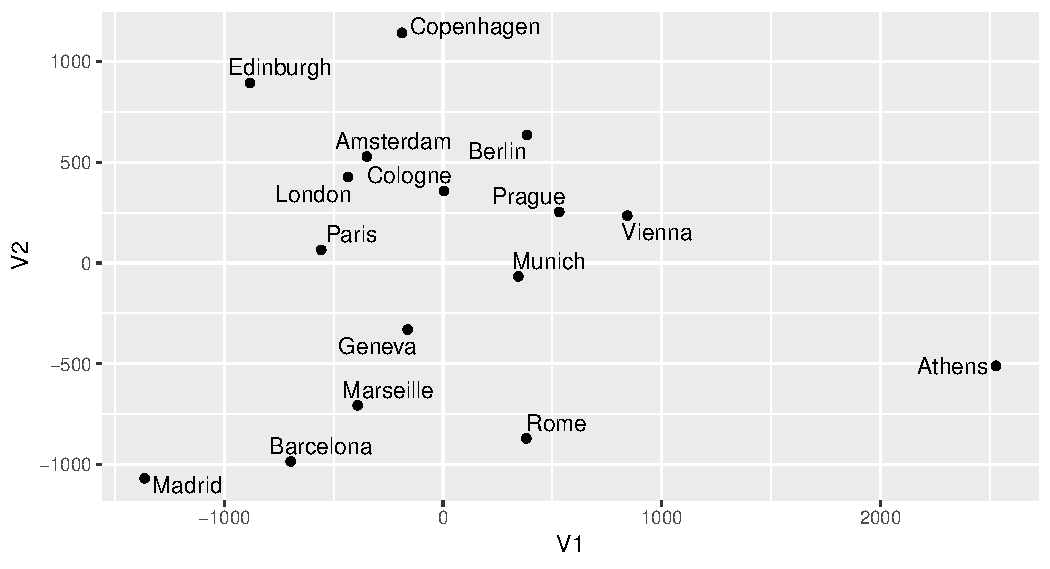
\includegraphics{figure/unnamed-chunk-10-1.pdf}
\caption{plot of chunk unnamed-chunk-10}
\end{figure}

\end{frame}

\begin{frame}[fragile]{Making a function}
\protect\hypertarget{making-a-function}{}

\begin{itemize}
\tightlist
\item
  Idea: given input distance matrix (as stored in a CSV file), output a
  map (like the one on the previous page). xxx
\end{itemize}

\scriptsize

\begin{Shaded}
\begin{Highlighting}[]
\NormalTok{mds_map <-}\StringTok{ }\ControlFlowTok{function}\NormalTok{(filename) \{}
\NormalTok{  x <-}\StringTok{ }\KeywordTok{read_csv}\NormalTok{(filename)}
\NormalTok{  dist <-}\StringTok{ }\NormalTok{x }\OperatorTok
\StringTok{    }\KeywordTok{select_if}\NormalTok{(is.numeric) }\OperatorTok
\StringTok{    }\KeywordTok{as.dist}\NormalTok{()}
\NormalTok{  x.scale <-}\StringTok{ }\KeywordTok{cmdscale}\NormalTok{(dist) }\CommentTok{# this is a matrix}
\NormalTok{  x_coord <-}\StringTok{ }\NormalTok{x.scale }\OperatorTok
\StringTok{    }\KeywordTok{as_tibble}\NormalTok{() }\OperatorTok
\StringTok{    }\KeywordTok{mutate}\NormalTok{(}\DataTypeTok{place =} \KeywordTok{row.names}\NormalTok{(x.scale))}
  \KeywordTok{ggplot}\NormalTok{(x_coord, }\KeywordTok{aes}\NormalTok{(}\DataTypeTok{x =}\NormalTok{ V1, }\DataTypeTok{y =}\NormalTok{ V2, }\DataTypeTok{label =}\NormalTok{ place)) }\OperatorTok{+}
\StringTok{    }\KeywordTok{geom_point}\NormalTok{() }\OperatorTok{+}\StringTok{ }\KeywordTok{geom_text_repel}\NormalTok{() }\OperatorTok{+}
\StringTok{    }\KeywordTok{coord_fixed}\NormalTok{()}
\NormalTok{\}}
\end{Highlighting}
\end{Shaded}

\normalsize

\begin{itemize}
\item
  Use \texttt{select\_if} to pick out all the numerical columns (no
  text), whichever they are.
\item
  \texttt{x.scale} is matrix with no column headers. Turn into data
  frame, acquires headers \texttt{V1} and \texttt{V2}.
\item
  Get place names from \texttt{cmdscale} output.
\end{itemize}

\end{frame}

\begin{frame}[fragile]{Does it work?}
\protect\hypertarget{does-it-work}{}

\begin{Shaded}
\begin{Highlighting}[]
\KeywordTok{mds_map}\NormalTok{(}\StringTok{"europe.csv"}\NormalTok{)}
\end{Highlighting}
\end{Shaded}

\begin{figure}
\centering
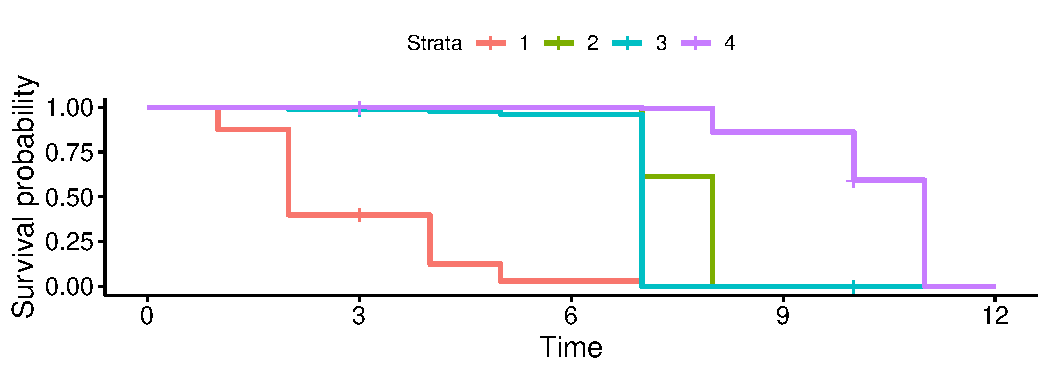
\includegraphics{figure/unnamed-chunk-12-1.pdf}
\caption{plot of chunk unnamed-chunk-12}
\end{figure}

\end{frame}

\begin{frame}[fragile]{A square xxx}
\protect\hypertarget{a-square-xxx}{}

\begin{minipage}[t]{0.5\textwidth}

The data, in `square.csv`:
\begin{small}

```
x,A  ,B  ,C  ,D
A,0  ,1  ,1  ,1.4
B,1  ,0  ,1.4,1
C,1  ,1.4,0  ,1
D,1.4,1  ,1  ,0
```
\end{small}
\end{minipage}\hfill

\textbackslash{}begin\{minipage\}{[}t{]}{[}{]}{[}b{]}\{0.48\textwidth\}
* The map (on right):

\begin{Shaded}
\begin{Highlighting}[]
\KeywordTok{mds_map}\NormalTok{(}\StringTok{"square.csv"}\NormalTok{)}
\end{Highlighting}
\end{Shaded}

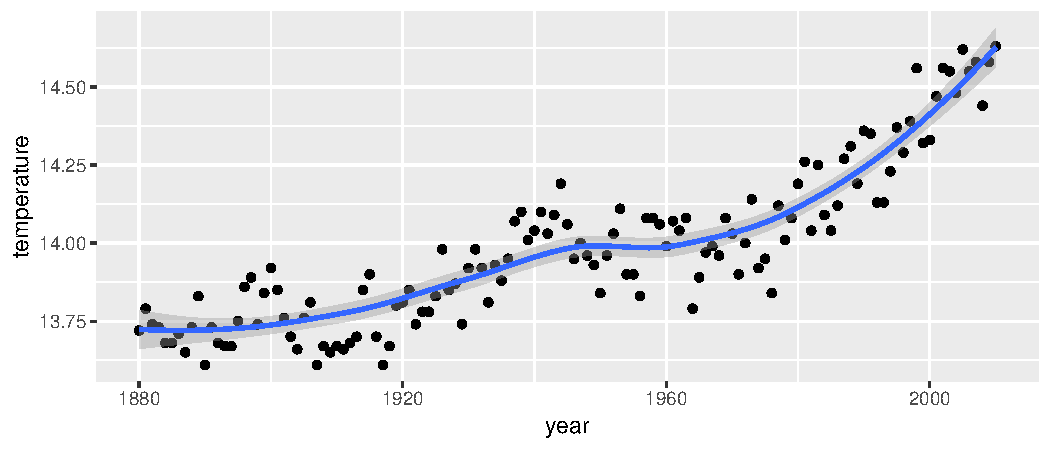
\includegraphics{figure/unnamed-chunk-13-1.pdf}
\textbackslash{}end\{minipage\}

\end{frame}

\begin{frame}[fragile]{Drawing a map of the real Europe}
\protect\hypertarget{drawing-a-map-of-the-real-europe}{}

\begin{itemize}
\item
  Works with package \texttt{ggmap}.
\item
  First find latitudes and longitudes of our cities, called
  \emph{geocoding}: xxx
\end{itemize}

\small

\begin{Shaded}
\begin{Highlighting}[]
\NormalTok{latlong <-}\StringTok{ }\KeywordTok{geocode}\NormalTok{(europe}\OperatorTok{$}\NormalTok{City)}
\NormalTok{latlong <-}\StringTok{ }\KeywordTok{bind_cols}\NormalTok{(}\DataTypeTok{city =}\NormalTok{ europe}\OperatorTok{$}\NormalTok{City, latlong)}
\NormalTok{latlong }\OperatorTok\StringTok{ }\KeywordTok{slice}\NormalTok{(}\DecValTok{1}\OperatorTok{:}\DecValTok{6}\NormalTok{)}
\end{Highlighting}
\end{Shaded}

\normalsize

xxx

\small

\begin{verbatim}
## # A tibble: 6 x 3
##   city         lon   lat
##   <chr>      <dbl> <dbl>
## 1 Amsterdam   4.90  52.4
## 2 Athens     23.7   38.0
## 3 Barcelona   2.17  41.4
## 4 Berlin     13.4   52.5
## 5 Cologne     6.96  50.9
## 6 Copenhagen 12.6   55.7
\end{verbatim}

\normalsize

\begin{itemize}
\tightlist
\item
  Just so you know, there is a limit of 2500 queries per day (it queries
  Google Maps).
\end{itemize}

\end{frame}

\begin{frame}[fragile]{Making the map}
\protect\hypertarget{making-the-map}{}

\begin{itemize}
\tightlist
\item
  Get a map of Europe from Google Maps (specify what you want a map of
  any way you can in Google Maps). This one centres the map on the city
  shown and zooms it so all the cities appear (I had to experiment):
\end{itemize}

\begin{Shaded}
\begin{Highlighting}[]
\NormalTok{map <-}\StringTok{ }\KeywordTok{get_map}\NormalTok{(}\StringTok{"Memmingen DE"}\NormalTok{, }\DataTypeTok{zoom =} \DecValTok{5}\NormalTok{)}
\end{Highlighting}
\end{Shaded}

\begin{itemize}
\tightlist
\item
  Plot the map with \texttt{ggmap}. This is \texttt{ggplot}, so add
  anything to it that you would add to a \texttt{ggplot}, such as cities
  we want to show:
\end{itemize}

\begin{Shaded}
\begin{Highlighting}[]
\NormalTok{g2 <-}\StringTok{ }\KeywordTok{ggmap}\NormalTok{(map) }\OperatorTok{+}
\StringTok{  }\KeywordTok{geom_point}\NormalTok{(}
    \DataTypeTok{data =}\NormalTok{ latlong, }\KeywordTok{aes}\NormalTok{(}\DataTypeTok{x =}\NormalTok{ lon, }\DataTypeTok{y =}\NormalTok{ lat),}
    \DataTypeTok{shape =} \DecValTok{3}\NormalTok{, }\DataTypeTok{colour =} \StringTok{"red"}
\NormalTok{  )}
\end{Highlighting}
\end{Shaded}

\begin{itemize}
\tightlist
\item
  We don't have a default data frame or \texttt{aes} for our
  \texttt{geom\_point}, so have to specify one.
\end{itemize}

\end{frame}

\begin{frame}[fragile]{The real Europe with our cities}
\protect\hypertarget{the-real-europe-with-our-cities}{}

\begin{Shaded}
\begin{Highlighting}[]
\NormalTok{g2}
\end{Highlighting}
\end{Shaded}

\begin{figure}
\centering
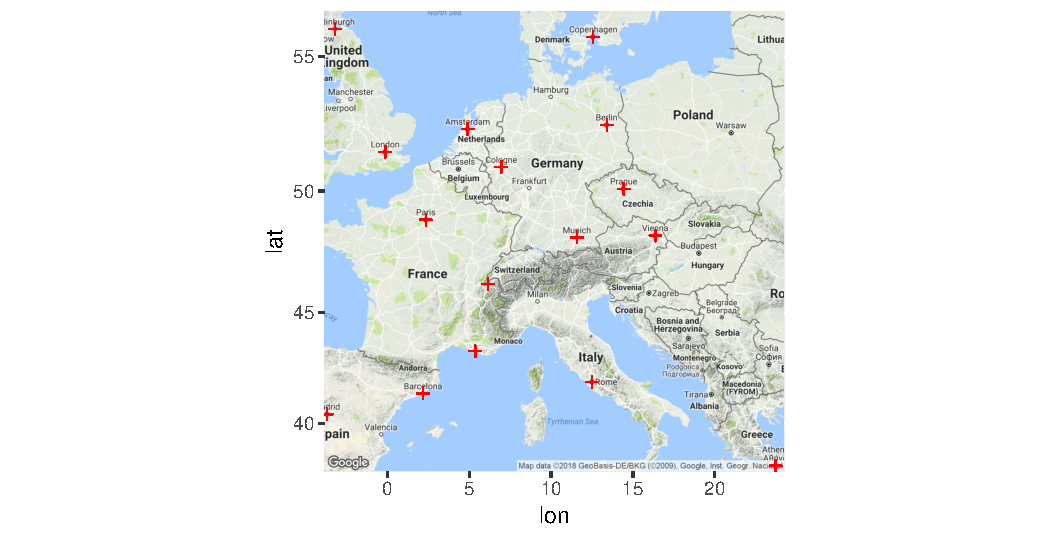
\includegraphics{figure/unnamed-chunk-19-1.pdf}
\caption{plot of chunk unnamed-chunk-19}
\end{figure}

\end{frame}

\begin{frame}{Compare our scaling map}
\protect\hypertarget{compare-our-scaling-map}{}

\begin{figure}
\centering
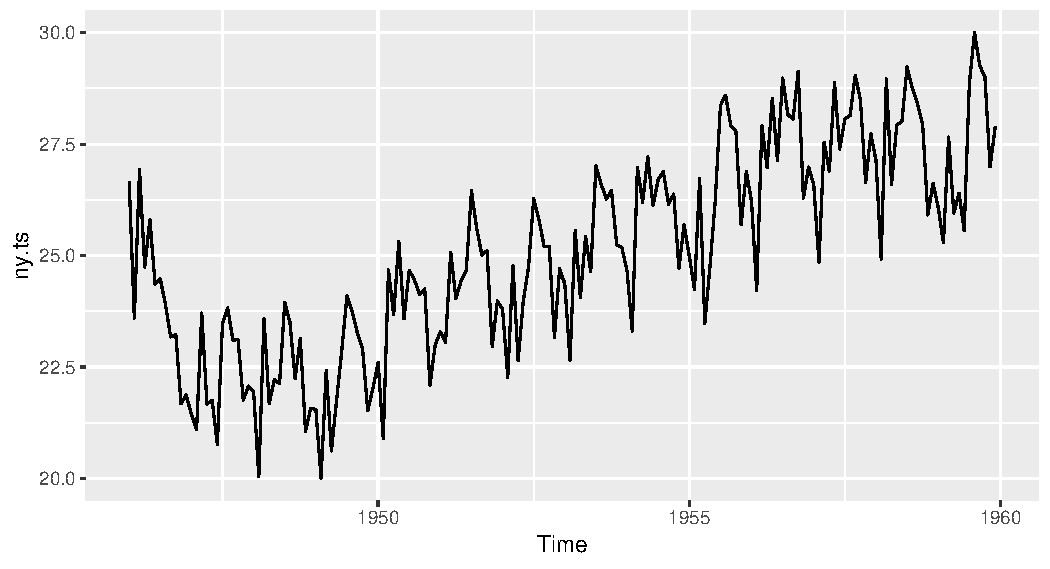
\includegraphics{figure/unnamed-chunk-20-1.pdf}
\caption{plot of chunk unnamed-chunk-20}
\end{figure}

\end{frame}

\begin{frame}{Comments}
\protect\hypertarget{comments}{}

\begin{itemize}
\item
  North-south not quite right: Edinburgh and Copenhagen on same
  latitude, also Amsterdam and Berlin; Athens should be south of Rome.
\item
  Rotating clockwise by about 45 degrees should fix that.
\item
  General point: MDS only uses distances, so answer can be ``off'' by
  rotation (as here) or reflection (flipping over, say exchanging west
  and east while leaving north and south same).
\end{itemize}

\end{frame}

\begin{frame}[fragile]{Exploring the map by plotting in 3 dimensions}
\protect\hypertarget{exploring-the-map-by-plotting-in-3-dimensions}{}

\begin{itemize}
\item
  Package \texttt{rgl} makes 3D plots.
\item
  We have to fake up a 3rd dimension (by setting all its values to 1).
\item
  Try this code:
\end{itemize}

\begin{Shaded}
\begin{Highlighting}[]
\KeywordTok{library}\NormalTok{(rgl)}
\NormalTok{es}\FloatTok{.2}\NormalTok{ <-}\StringTok{ }\KeywordTok{cbind}\NormalTok{(europe.scale, }\DecValTok{1}\NormalTok{)}
\KeywordTok{plot3d}\NormalTok{(es}\FloatTok{.2}\NormalTok{, }\DataTypeTok{zlim =} \KeywordTok{c}\NormalTok{(}\OperatorTok{-}\DecValTok{1000}\NormalTok{, }\DecValTok{1000}\NormalTok{))}
\KeywordTok{text3d}\NormalTok{(es}\FloatTok{.2}\NormalTok{, }\DataTypeTok{text =}\NormalTok{ d}\OperatorTok{$}\NormalTok{city)}
\end{Highlighting}
\end{Shaded}

\begin{itemize}
\item
  Opens a graphics window with the cities plotted and named.
\item
  Click and hold left mouse button to rotate plot. ``Rotate away'' 3rd
  dimension to get a possible map (that preserves distances).
\end{itemize}

\end{frame}

\begin{frame}[fragile]{Ontario, the same way}
\protect\hypertarget{ontario-the-same-way}{}

\ldots using our function: xxx

\begin{Shaded}
\begin{Highlighting}[]
\NormalTok{url <-}\StringTok{ }
\StringTok{  "http://www.utsc.utoronto.ca/~butler/d29/ontario-road-distances.csv"}
\NormalTok{g <-}\StringTok{ }\KeywordTok{mds_map}\NormalTok{(url)}
\NormalTok{g}
\end{Highlighting}
\end{Shaded}

\begin{figure}
\centering
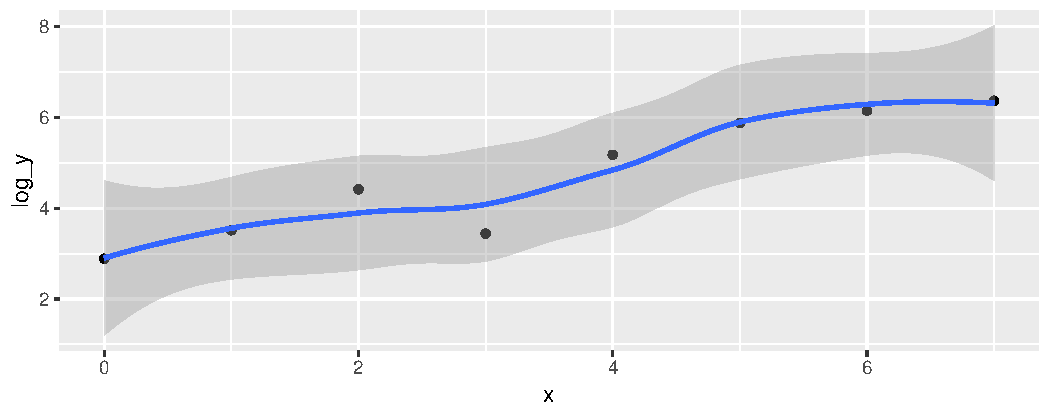
\includegraphics{figure/unnamed-chunk-22-1.pdf}
\caption{plot of chunk unnamed-chunk-22}
\end{figure}

Thunder Bay and Sault Ste Marie dominate the picture since they are so
far away from everywhere else. \textless{}\textgreater{}=
ontario=read.csv(``ontario-road-distances.csv'',header=T)
ontario.d=as.dist(ontario) ontario.scale=cmdscale(ontario.d)
d=data.frame(ontario.scale,city=colnames(ontario))
g=ggplot(d,aes(x=X1,y=X2,label=city))+ geom\_point()+coord\_fixed()+
geom\_text\_repel() @

\end{frame}

\begin{frame}{Removing points}
\protect\hypertarget{removing-points}{}

\begin{itemize}
\item
  Messy: have to find which rows and columns contain those cities, then
  remove just those rows and columns.
\item
  Better:
\item
  ``tidy'' the distance matrix
\item
  then remove rows we don't need
\item
  then ``untidy'' it again
\item
  save into .csv file
\item
  Illustrate with square data first (easier to see).
\end{itemize}

\end{frame}

\begin{frame}[fragile]{Square data}
\protect\hypertarget{square-data}{}

\begin{Shaded}
\begin{Highlighting}[]
\NormalTok{my_url <-}\StringTok{ "http://www.utsc.utoronto.ca/~butler/d29/square.csv"}
\NormalTok{square <-}\StringTok{ }\KeywordTok{read_csv}\NormalTok{(my_url)}
\NormalTok{square}
\end{Highlighting}
\end{Shaded}

\begin{verbatim}
## # A tibble: 4 x 5
##   x         A     B     C     D
##   <chr> <dbl> <dbl> <dbl> <dbl>
## 1 A       0     1     1     1.4
## 2 B       1     0     1.4   1  
## 3 C       1     1.4   0     1  
## 4 D       1.4   1     1     0
\end{verbatim}

\end{frame}

\begin{frame}[fragile]{Make tidy xxx}
\protect\hypertarget{make-tidy-xxx}{}

\scriptsize

\begin{Shaded}
\begin{Highlighting}[]
\NormalTok{square }\OperatorTok\StringTok{ }\KeywordTok{gather}\NormalTok{(point, distance, }\OperatorTok{-}\NormalTok{x)}
\end{Highlighting}
\end{Shaded}

\begin{verbatim}
## # A tibble: 16 x 3
##    x     point distance
##    <chr> <chr>    <dbl>
##  1 A     A          0  
##  2 B     A          1  
##  3 C     A          1  
##  4 D     A          1.4
##  5 A     B          1  
##  6 B     B          0  
##  7 C     B          1.4
##  8 D     B          1  
##  9 A     C          1  
## 10 B     C          1.4
## 11 C     C          0  
## 12 D     C          1  
## 13 A     D          1.4
## 14 B     D          1  
## 15 C     D          1  
## 16 D     D          0
\end{verbatim}

\normalsize

\end{frame}

\begin{frame}[fragile]{Remove all references to point C}
\protect\hypertarget{remove-all-references-to-point-c}{}

In column \texttt{x} or \texttt{point}: xxx

\small

\begin{Shaded}
\begin{Highlighting}[]
\NormalTok{square }\OperatorTok
\StringTok{  }\KeywordTok{gather}\NormalTok{(point, distance, }\DecValTok{-1}\NormalTok{) }\OperatorTok
\StringTok{  }\KeywordTok{filter}\NormalTok{(x }\OperatorTok{!=}\StringTok{ "C"}\NormalTok{, point }\OperatorTok{!=}\StringTok{ "C"}\NormalTok{)}
\end{Highlighting}
\end{Shaded}

\begin{verbatim}
## # A tibble: 9 x 3
##   x     point distance
##   <chr> <chr>    <dbl>
## 1 A     A          0  
## 2 B     A          1  
## 3 D     A          1.4
## 4 A     B          1  
## 5 B     B          0  
## 6 D     B          1  
## 7 A     D          1.4
## 8 B     D          1  
## 9 D     D          0
\end{verbatim}

\normalsize

\end{frame}

\begin{frame}[fragile]{Put back as distance matrix}
\protect\hypertarget{put-back-as-distance-matrix}{}

and save as .csv when we are happy:

\begin{Shaded}
\begin{Highlighting}[]
\NormalTok{noc <-}\StringTok{ }\NormalTok{square }\OperatorTok
\StringTok{  }\KeywordTok{gather}\NormalTok{(point, distance, }\DecValTok{-1}\NormalTok{) }\OperatorTok
\StringTok{  }\KeywordTok{filter}\NormalTok{(x }\OperatorTok{!=}\StringTok{ "C"}\NormalTok{, point }\OperatorTok{!=}\StringTok{ "C"}\NormalTok{) }\OperatorTok
\StringTok{  }\KeywordTok{spread}\NormalTok{(point, distance)}
\NormalTok{noc}
\end{Highlighting}
\end{Shaded}

\begin{verbatim}
## # A tibble: 3 x 4
##   x         A     B     D
##   <chr> <dbl> <dbl> <dbl>
## 1 A       0       1   1.4
## 2 B       1       0   1  
## 3 D       1.4     1   0
\end{verbatim}

\begin{Shaded}
\begin{Highlighting}[]
\NormalTok{noc }\OperatorTok\StringTok{ }\KeywordTok{write_csv}\NormalTok{(}\StringTok{"no-c.csv"}\NormalTok{)}
\end{Highlighting}
\end{Shaded}

\end{frame}

\begin{frame}[fragile]{Make map of square-without-C}
\protect\hypertarget{make-map-of-square-without-c}{}

\begin{Shaded}
\begin{Highlighting}[]
\KeywordTok{mds_map}\NormalTok{(}\StringTok{"no-c.csv"}\NormalTok{)}
\end{Highlighting}
\end{Shaded}

\begin{figure}
\centering
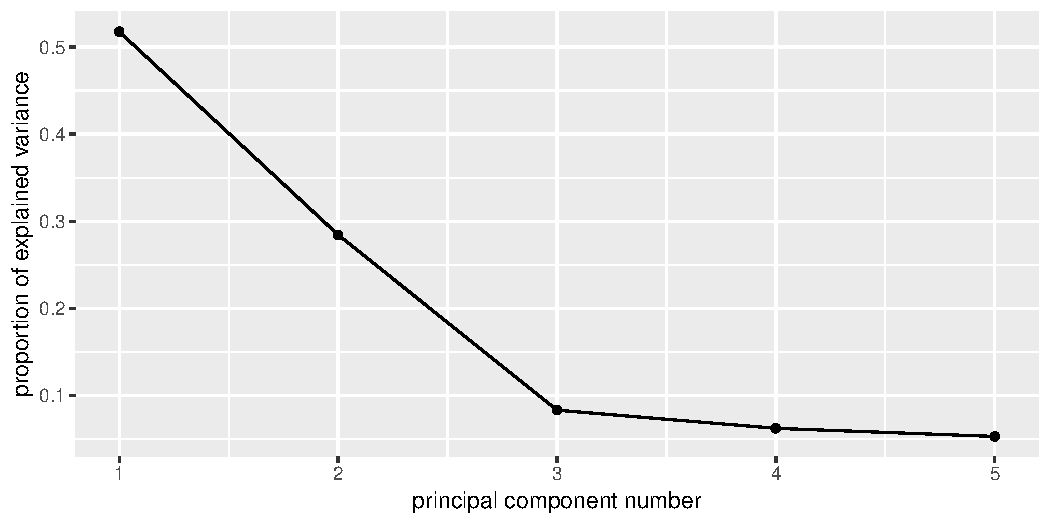
\includegraphics{figure/unnamed-chunk-27-1.pdf}
\caption{plot of chunk unnamed-chunk-27}
\end{figure}

\end{frame}

\begin{frame}[fragile]{Back to Ontario}
\protect\hypertarget{back-to-ontario}{}

\begin{Shaded}
\begin{Highlighting}[]
\NormalTok{g}
\end{Highlighting}
\end{Shaded}

\begin{figure}
\centering
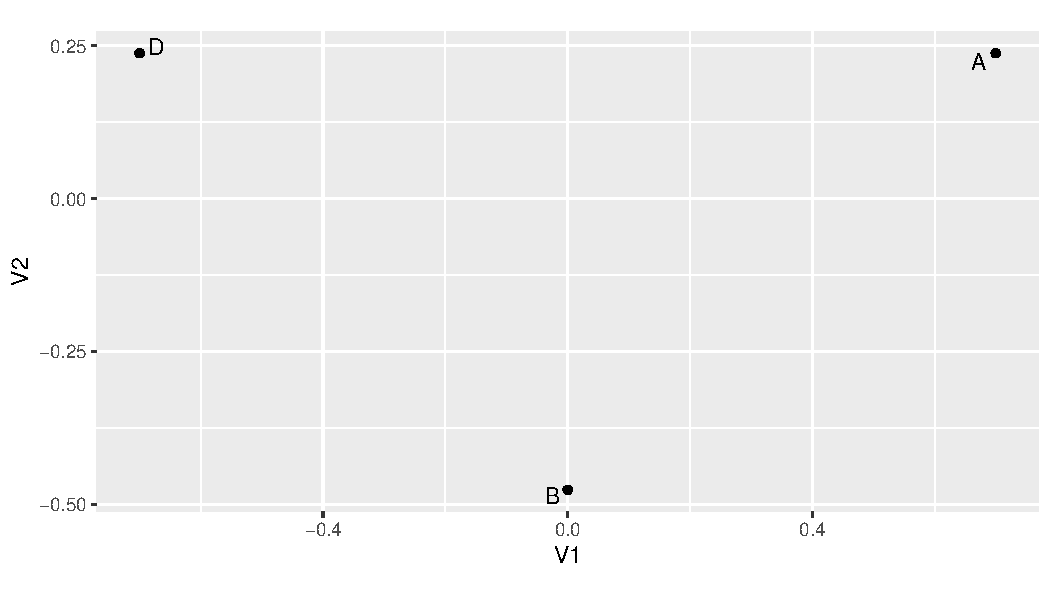
\includegraphics{figure/unnamed-chunk-28-1.pdf}
\caption{plot of chunk unnamed-chunk-28}
\end{figure}

Get rid of Thunder Bay and Sault Ste Marie.

\end{frame}

\begin{frame}[fragile]{Tidy, remove, untidy xxx}
\protect\hypertarget{tidy-remove-untidy-xxx}{}

\footnotesize

\begin{Shaded}
\begin{Highlighting}[]
\NormalTok{my_url <-}\StringTok{ }
\StringTok{  "http://www.utsc.utoronto.ca/~butler/d29/ontario-road-distances.csv"}
\NormalTok{ontario2 <-}\StringTok{ }\KeywordTok{read_csv}\NormalTok{(my_url) }
\NormalTok{ontario2 }\OperatorTok
\StringTok{  }\KeywordTok{gather}\NormalTok{(city, distance, }\DecValTok{-1}\NormalTok{) }\OperatorTok
\StringTok{  }\KeywordTok{filter}\NormalTok{(}
\NormalTok{    city }\OperatorTok{!=}\StringTok{ "Thunder Bay"}\NormalTok{,}
\NormalTok{    place }\OperatorTok{!=}\StringTok{ "Thunder Bay"}\NormalTok{,}
\NormalTok{    city }\OperatorTok{!=}\StringTok{ "Sault Ste Marie"}\NormalTok{,}
\NormalTok{    place }\OperatorTok{!=}\StringTok{ "Sault Ste Marie"}
\NormalTok{  ) }\OperatorTok
\StringTok{  }\KeywordTok{spread}\NormalTok{(place, distance) }\OperatorTok
\StringTok{  }\KeywordTok{write_csv}\NormalTok{(}\StringTok{"southern-ontario.csv"}\NormalTok{)}
\end{Highlighting}
\end{Shaded}

\normalsize

\end{frame}

\begin{frame}[fragile]{Map of Southern Ontario}
\protect\hypertarget{map-of-southern-ontario}{}

\begin{Shaded}
\begin{Highlighting}[]
\NormalTok{g <-}\StringTok{ }\KeywordTok{mds_map}\NormalTok{(}\StringTok{"southern-ontario.csv"}\NormalTok{)}
\NormalTok{g}
\end{Highlighting}
\end{Shaded}

\begin{figure}
\centering
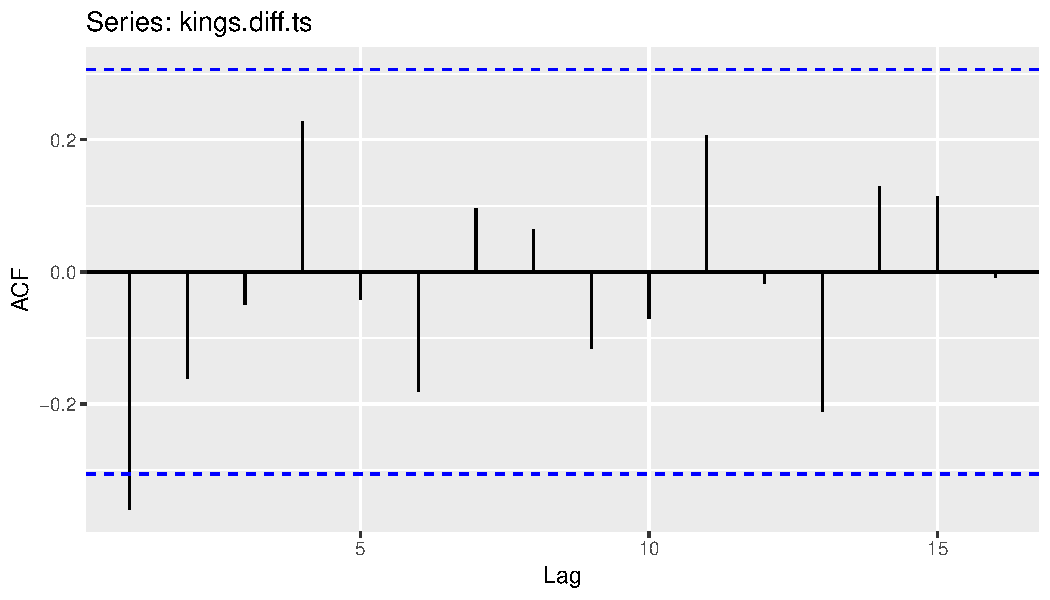
\includegraphics{figure/unnamed-chunk-30-1.pdf}
\caption{plot of chunk unnamed-chunk-30}
\end{figure}

Came out geographically about right.

\end{frame}

\begin{frame}[fragile]{What about that cluster of points?}
\protect\hypertarget{what-about-that-cluster-of-points}{}

\begin{itemize}
\item
  Plot looks generally good, but what about that cluster of points?
\item
  ``Zoom in'' on area between \(-150\) and \(-100\) on \(x\) axis,
  \(-50\) to 0 on \(y\) axis.
\item
  Code below overrides the \texttt{coord\_fixed} we had before. xxx
\end{itemize}

\small

\begin{Shaded}
\begin{Highlighting}[]
\NormalTok{g2 <-}\StringTok{ }\NormalTok{g }\OperatorTok{+}\StringTok{ }\KeywordTok{coord_fixed}\NormalTok{(}\DataTypeTok{xlim =} \KeywordTok{c}\NormalTok{(}\OperatorTok{-}\DecValTok{150}\NormalTok{, }\DecValTok{-100}\NormalTok{), }\DataTypeTok{ylim =} \KeywordTok{c}\NormalTok{(}\OperatorTok{-}\DecValTok{50}\NormalTok{, }\DecValTok{0}\NormalTok{))}
\end{Highlighting}
\end{Shaded}

\begin{verbatim}
## Coordinate system already present. Adding new coordinate system, which will replace the existing one.
\end{verbatim}

\normalsize

\end{frame}

\begin{frame}[fragile]{Zoomed-in plot}
\protect\hypertarget{zoomed-in-plot}{}

Ignore the arrows to points off the map:

\begin{Shaded}
\begin{Highlighting}[]
\NormalTok{g2}
\end{Highlighting}
\end{Shaded}

\begin{figure}
\centering
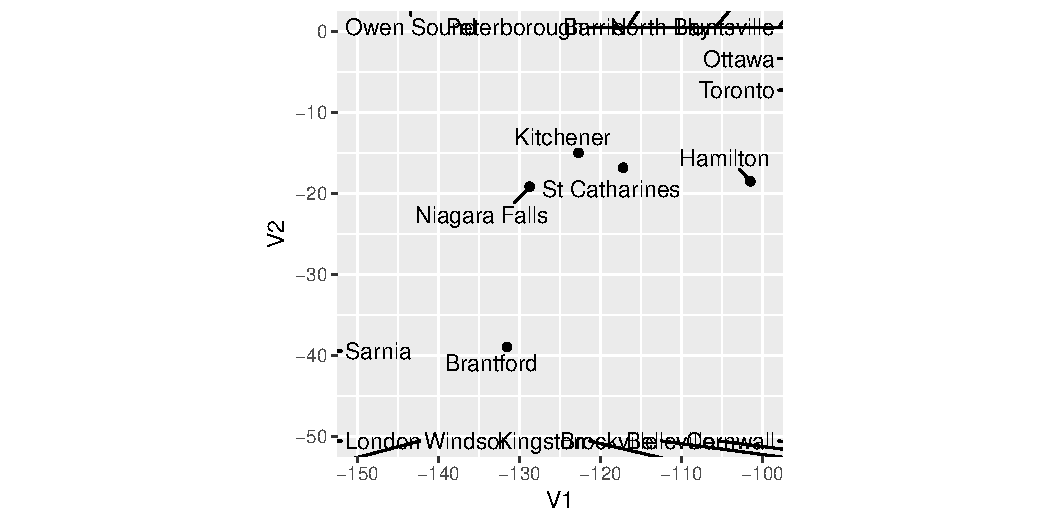
\includegraphics{figure/spal-1.pdf}
\caption{plot of chunk spal}
\end{figure}

\end{frame}

\begin{frame}[fragile]{Does that make sense?}
\protect\hypertarget{does-that-make-sense}{}

\begin{itemize}
\item
  Get a Google map of the area, with the points labelled.
\item
  First geocode the cities of interest: xxx
\end{itemize}

\footnotesize

\begin{Shaded}
\begin{Highlighting}[]
\NormalTok{cities <-}\StringTok{ }\KeywordTok{c}\NormalTok{(}
  \StringTok{"Kitchener ON"}\NormalTok{, }\StringTok{"Hamilton ON"}\NormalTok{, }\StringTok{"Niagara Falls ON"}\NormalTok{,}
  \StringTok{"St Catharines ON"}\NormalTok{, }\StringTok{"Brantford ON"}
\NormalTok{)}
\NormalTok{latlong <-}\StringTok{ }\KeywordTok{geocode}\NormalTok{(cities)}
\NormalTok{latlong <-}\StringTok{ }\KeywordTok{bind_cols}\NormalTok{(}\DataTypeTok{city =}\NormalTok{ cities, latlong) }\OperatorTok\StringTok{ }\KeywordTok{print}\NormalTok{()}
\end{Highlighting}
\end{Shaded}

\begin{verbatim}
## # A tibble: 5 x 3
##   city               lon   lat
##   <chr>            <dbl> <dbl>
## 1 Kitchener ON     -80.5  43.5
## 2 Hamilton ON      -79.9  43.3
## 3 Niagara Falls ON -79.1  43.1
## 4 St Catharines ON -79.2  43.2
## 5 Brantford ON     -80.3  43.1
\end{verbatim}

\normalsize

\begin{itemize}
\tightlist
\item
  Get a Google map of the area (experiment with zoom):
\end{itemize}

\begin{Shaded}
\begin{Highlighting}[]
\NormalTok{map <-}\StringTok{ }\KeywordTok{get_map}\NormalTok{(}\StringTok{"Hamilton ON"}\NormalTok{, }\DataTypeTok{zoom =} \DecValTok{8}\NormalTok{)}
\end{Highlighting}
\end{Shaded}

get from file

\begin{itemize}
\tightlist
\item
  Plot map with cities marked.
\end{itemize}

\end{frame}

\begin{frame}[fragile]{Making the Google map}
\protect\hypertarget{making-the-google-map}{}

Plot the map, plus the cities, plus labels for the cities:

\begin{Shaded}
\begin{Highlighting}[]
\KeywordTok{ggmap}\NormalTok{(map) }\OperatorTok{+}
\StringTok{  }\KeywordTok{geom_point}\NormalTok{(}
    \DataTypeTok{data =}\NormalTok{ latlong,}
    \KeywordTok{aes}\NormalTok{(}\DataTypeTok{x =}\NormalTok{ lon, }\DataTypeTok{y =}\NormalTok{ lat),}
    \DataTypeTok{shape =} \DecValTok{3}\NormalTok{, }\DataTypeTok{colour =} \StringTok{"red"}
\NormalTok{  ) }\OperatorTok{+}
\StringTok{  }\KeywordTok{geom_text_repel}\NormalTok{(}
    \DataTypeTok{data =}\NormalTok{ latlong,}
    \KeywordTok{aes}\NormalTok{(}\DataTypeTok{label =}\NormalTok{ city)}
\NormalTok{  ) ->}\StringTok{ }\NormalTok{gmap}
\end{Highlighting}
\end{Shaded}

\textbackslash{}begin\{frame\}{[}frame{]}\{The \texttt{mds} map and
Google map\}

\begin{multicols}{2}

```r
g2
```

![plot of chunk unnamed-chunk-36](figure/unnamed-chunk-36-1.pdf)

     


```r
gmap
```

![plot of chunk unnamed-chunk-37](figure/unnamed-chunk-37-1.pdf)

 
\end{multicols}

St Catharines and Niagara Falls should be the \emph{other} side of
Hamilton!

\end{frame}

\begin{frame}[fragile]{Quality of fit}
\protect\hypertarget{quality-of-fit}{}

\begin{itemize}
\tightlist
\item
  Read in ``southern Ontario'' data set from file:
\end{itemize}

\begin{Shaded}
\begin{Highlighting}[]
\NormalTok{my_url <-}\StringTok{ "http://www.utsc.utoronto.ca/~butler/d29/southern-ontario.csv"}
\NormalTok{ontario2 <-}\StringTok{ }\KeywordTok{read_csv}\NormalTok{(my_url)}
\end{Highlighting}
\end{Shaded}

\begin{itemize}
\tightlist
\item
  Calling \texttt{cmdscale} with \texttt{eig=T} gives more info: xxx
\end{itemize}

\footnotesize

\begin{Shaded}
\begin{Highlighting}[]
\NormalTok{ontario2}\FloatTok{.2}\NormalTok{ <-}\StringTok{ }\NormalTok{ontario2 }\OperatorTok
\StringTok{  }\KeywordTok{select_if}\NormalTok{(is.numeric) }\OperatorTok
\StringTok{  }\KeywordTok{cmdscale}\NormalTok{(}\DataTypeTok{eig =}\NormalTok{ T)}
\KeywordTok{names}\NormalTok{(ontario2}\FloatTok{.2}\NormalTok{)}
\end{Highlighting}
\end{Shaded}

\begin{verbatim}
## [1] "points" "eig"    "x"      "ac"     "GOF"
\end{verbatim}

\begin{Shaded}
\begin{Highlighting}[]
\NormalTok{ontario2}\FloatTok{.2}\OperatorTok{$}\NormalTok{GOF}
\end{Highlighting}
\end{Shaded}

\begin{verbatim}
## [1] 0.8381590 0.8914059
\end{verbatim}

\begin{Shaded}
\begin{Highlighting}[]
\NormalTok{ontario2}\FloatTok{.3}\NormalTok{ <-}\StringTok{ }\NormalTok{ontario2 }\OperatorTok
\StringTok{  }\KeywordTok{select_if}\NormalTok{(is.numeric) }\OperatorTok
\StringTok{  }\KeywordTok{cmdscale}\NormalTok{(}\DecValTok{3}\NormalTok{, }\DataTypeTok{eig =}\NormalTok{ T)}
\NormalTok{ontario2}\FloatTok{.3}\OperatorTok{$}\NormalTok{GOF}
\end{Highlighting}
\end{Shaded}

\begin{verbatim}
## [1] 0.8852559 0.9414948
\end{verbatim}

\normalsize

\end{frame}

\begin{frame}[fragile]{Comments}
\protect\hypertarget{comments-1}{}

\begin{itemize}
\item
  Coordinates now in \texttt{points}.
\item
  \texttt{GOF} is R-squared-like measure saying how well map distances
  match real ones. Higher is better.
\item
  For Ontario road distances, \texttt{GOF} better for 3 dimensions than
  2, presumably to accommodate St Catharines and Niagara Falls?
\end{itemize}

\end{frame}

\begin{frame}[fragile]{3-dimensional coordinates, cities attached xxx}
\protect\hypertarget{dimensional-coordinates-cities-attached-xxx}{}

\scriptsize

\begin{Shaded}
\begin{Highlighting}[]
\NormalTok{ontario2}\FloatTok{.3}\OperatorTok{$}\NormalTok{points }\OperatorTok
\StringTok{  }\KeywordTok{as_tibble}\NormalTok{() }\OperatorTok
\StringTok{  }\KeywordTok{mutate}\NormalTok{(}\DataTypeTok{city =}\NormalTok{ ontario2}\OperatorTok{$}\NormalTok{x)}
\end{Highlighting}
\end{Shaded}

\begin{verbatim}
## # A tibble: 19 x 4
##        V1       V2      V3 city         
##     <dbl>    <dbl>   <dbl> <chr>        
##  1  -38.7  122.       4.17 Barrie       
##  2  146.   -82.8      1.53 Belleville   
##  3 -132.   -38.9     14.1  Brantford    
##  4  298.  -106.      -7.74 Brockville   
##  5  397.  -104.     -22.0  Cornwall     
##  6 -101.   -18.5     30.0  Hamilton     
##  7   62.4  198.     -14.0  Huntsville   
##  8  214.  -129.      10.8  Kingston     
##  9 -123.   -15.0     -6.44 Kitchener    
## 10 -208.   -51.6    -36.5  London       
## 11 -129.   -19.1    155.   Niagara Falls
## 12  146.   300.     -25.4  North Bay    
## 13  368.    -4.30   -47.2  Ottawa       
## 14 -145.   125.     -16.0  Owen Sound   
## 15   82.5    0.551   -6.92 Peterborough 
## 16 -299.   -39.4    -72.5  Sarnia       
## 17 -117.   -16.8    123.   St Catharines
## 18  -34.3   -4.75    15.8  Toronto      
## 19 -388.  -116.     -99.5  Windsor
\end{verbatim}

\normalsize

\end{frame}

\begin{frame}[fragile]{RGL code for 3 dimensions}
\protect\hypertarget{rgl-code-for-3-dimensions}{}

\begin{Shaded}
\begin{Highlighting}[]
\KeywordTok{library}\NormalTok{(rgl)}
\KeywordTok{plot3d}\NormalTok{(ontario}\FloatTok{.3}\NormalTok{)}
\KeywordTok{text3d}\NormalTok{(ontario}\FloatTok{.3}\NormalTok{, }\DataTypeTok{text =}\NormalTok{ d2}\OperatorTok{$}\NormalTok{city)}
\end{Highlighting}
\end{Shaded}

\textbackslash{}begin\{frame\}{[}fragile{]}\{Comparing MDS solution with
``reality'': Procrustes rotation\}

\begin{itemize}
\item
  How to tell that an MDS map makes a good correspondence with ``what
  should be''?
\item
  Problem: MDS map might be rotated/scaled/reflected from reality.
\item
  How to find rotation/scaling/reflection that best matches reality?
\item
  Answer: \textbf{Procrustes rotation}.
\item
  In R: \texttt{procOPA} in package \texttt{shapes}.
\end{itemize}

\end{frame}

\begin{frame}[fragile]{``True'' coordinates}
\protect\hypertarget{true-coordinates}{}

\begin{itemize}
\tightlist
\item
  Get latitudes and longitudes of cities by geocoding, as before. Glue
  ``ON'' onto city names to make sure we get right ones: xxx
\end{itemize}

\footnotesize

\begin{Shaded}
\begin{Highlighting}[]
\NormalTok{lookup <-}\StringTok{ }\KeywordTok{str_c}\NormalTok{(ontario2}\OperatorTok{$}\NormalTok{x, }\StringTok{" ON"}\NormalTok{)}
\NormalTok{latlong <-}\StringTok{ }\KeywordTok{geocode}\NormalTok{(lookup)}
\NormalTok{latlong <-}\StringTok{ }\KeywordTok{bind_cols}\NormalTok{(}\DataTypeTok{city =}\NormalTok{ ontario2}\OperatorTok{$}\NormalTok{x, latlong) }\OperatorTok\StringTok{ }\KeywordTok{print}\NormalTok{(}\DataTypeTok{n =} \DecValTok{4}\NormalTok{)}
\end{Highlighting}
\end{Shaded}

\normalsize

xxx

\footnotesize

\begin{verbatim}
## # A tibble: 19 x 3
##   city         lon   lat
##   <chr>      <dbl> <dbl>
## 1 Barrie     -79.7  44.4
## 2 Belleville -77.4  44.2
## 3 Brantford  -80.3  43.1
## 4 Brockville -75.7  44.6
## # … with 15 more rows
\end{verbatim}

\normalsize

\begin{itemize}
\tightlist
\item
  Not \((x,y)\) coordinates: one degree of latitude is always 110.25 km,
  but one degree of longitude is only that at the equator (less than
  that as you move further north, down to 0 km at north pole).
\end{itemize}

\end{frame}

\begin{frame}[fragile]{``True'' coordinates part 2}
\protect\hypertarget{true-coordinates-part-2}{}

\begin{itemize}
\item
  Make coordinates by multiplying by cosine of ``typical'' latitude.
\item
  Find mean latitude:
\end{itemize}

\begin{Shaded}
\begin{Highlighting}[]
\NormalTok{m <-}\StringTok{ }\KeywordTok{mean}\NormalTok{(latlong}\OperatorTok{$}\NormalTok{lat)}
\NormalTok{m}
\end{Highlighting}
\end{Shaded}

\begin{verbatim}
## [1] 44.01851
\end{verbatim}

\begin{itemize}
\tightlist
\item
  Turn into radians and find its cosine:
\end{itemize}

\begin{Shaded}
\begin{Highlighting}[]
\NormalTok{mult <-}\StringTok{ }\KeywordTok{cos}\NormalTok{(m }\OperatorTok{*}\StringTok{ }\NormalTok{pi }\OperatorTok{/}\StringTok{ }\DecValTok{180}\NormalTok{)}
\NormalTok{mult}
\end{Highlighting}
\end{Shaded}

\begin{verbatim}
## [1] 0.7191153
\end{verbatim}

\begin{itemize}
\tightlist
\item
  Create ``true'' coords by multiplying the longitudes by that. This
  needs to be R \texttt{matrix}, not data frame: xxx
\end{itemize}

\footnotesize

\begin{Shaded}
\begin{Highlighting}[]
\NormalTok{truecoord <-}\StringTok{ }\KeywordTok{with}\NormalTok{(latlong, }\KeywordTok{cbind}\NormalTok{(}\DataTypeTok{V1 =}\NormalTok{ lon }\OperatorTok{*}\StringTok{ }\NormalTok{mult, }\DataTypeTok{V2 =}\NormalTok{ lat))}
\end{Highlighting}
\end{Shaded}

\normalsize

\end{frame}

\begin{frame}[fragile]{Using \texttt{procOPA}}
\protect\hypertarget{using-procopa}{}

\begin{itemize}
\item
  Feed 2 things into \texttt{procOPA}: first, ``true'' coordinates,
  second MDS coordinates.
\item
  Get out:
\item
\begin{verbatim}
(centred and scaled) first set of coordinates `Ahat`
\end{verbatim}
\item
  (centred and scaled) second set of coordinates \texttt{Bhat}
\item
  sum of squared differences between two sets of coordinates
  \texttt{OSS}
\item
  Rotation matrix \texttt{R}
\item
  \texttt{Ahat} and \texttt{Bhat} coordinates supposed to match as well
  as possible. xxx
\end{itemize}

\footnotesize

\begin{Shaded}
\begin{Highlighting}[]
\NormalTok{ontario.pro <-}\StringTok{ }\KeywordTok{procOPA}\NormalTok{(}
\NormalTok{  truecoord,}
\NormalTok{  ontario2}\FloatTok{.2}\OperatorTok{$}\NormalTok{points}
\NormalTok{)}
\KeywordTok{names}\NormalTok{(ontario.pro)}
\end{Highlighting}
\end{Shaded}

\begin{verbatim}
## [1] "R"    "s"    "Ahat" "Bhat" "OSS"  "rmsd"
\end{verbatim}

\normalsize

\end{frame}

\begin{frame}[fragile]{Make data frames of output, glue together}
\protect\hypertarget{make-data-frames-of-output-glue-together}{}

\begin{itemize}
\tightlist
\item
  Two sets of coordinates, \texttt{Ahat} are actual, \texttt{Bhat} are
  from MDS. xxx
\end{itemize}

\scriptsize

\begin{Shaded}
\begin{Highlighting}[]
\NormalTok{A <-}\StringTok{ }\NormalTok{ontario.pro}\OperatorTok{$}\NormalTok{Ahat }\OperatorTok
\StringTok{  }\KeywordTok{as_tibble}\NormalTok{() }\OperatorTok
\StringTok{  }\KeywordTok{mutate}\NormalTok{(}\DataTypeTok{which =} \StringTok{"actual"}\NormalTok{, }\DataTypeTok{city =}\NormalTok{ ontario2}\OperatorTok{$}\NormalTok{x)}
\NormalTok{B <-}\StringTok{ }\NormalTok{ontario.pro}\OperatorTok{$}\NormalTok{Bhat }\OperatorTok
\StringTok{  }\KeywordTok{as_tibble}\NormalTok{() }\OperatorTok
\StringTok{  }\KeywordTok{mutate}\NormalTok{(}\DataTypeTok{which =} \StringTok{"MDS"}\NormalTok{, }\DataTypeTok{city =}\NormalTok{ ontario2}\OperatorTok{$}\NormalTok{x)}
\NormalTok{dp <-}\StringTok{ }\KeywordTok{bind_rows}\NormalTok{(A, B)}
\NormalTok{dp }\OperatorTok\StringTok{ }\KeywordTok{sample_n}\NormalTok{(}\DecValTok{6}\NormalTok{)}
\end{Highlighting}
\end{Shaded}

\begin{verbatim}
## # A tibble: 6 x 4
##       V1     V2 which  city        
##    <dbl>  <dbl> <chr>  <chr>       
## 1  1.87   0.213 actual Kingston    
## 2  0.556  0.298 MDS    Peterborough
## 3  2.45   0.571 actual Brockville  
## 4 -0.848 -0.879 actual Brantford   
## 5  2.39   0.348 MDS    Brockville  
## 6 -0.284  1.56  MDS    Huntsville
\end{verbatim}

\normalsize

\#\# \texttt{procOPA}, part 2: plotting

\begin{itemize}
\tightlist
\item
  Make data frames of each, glue together: xxx
\end{itemize}

\small

\begin{Shaded}
\begin{Highlighting}[]
\NormalTok{A=}\KeywordTok{with}\NormalTok{(ontario.pro,}\KeywordTok{data.frame}\NormalTok{(}\DataTypeTok{x=}\NormalTok{Ahat[,}\DecValTok{1}\NormalTok{],}
   \DataTypeTok{y=}\NormalTok{Ahat[,}\DecValTok{2}\NormalTok{],}\DataTypeTok{which=}\StringTok{"actual"}\NormalTok{,}\DataTypeTok{city=}\NormalTok{ontario2}\OperatorTok{$}\NormalTok{x)) }
\NormalTok{ B=}\KeywordTok{with}\NormalTok{(ontario.pro,}\KeywordTok{data.frame}\NormalTok{(}\DataTypeTok{x=}\NormalTok{Bhat[,}\DecValTok{1}\NormalTok{],}
   \DataTypeTok{y=}\NormalTok{Bhat[,}\DecValTok{2}\NormalTok{],}\DataTypeTok{which=}\StringTok{"MDS"}\NormalTok{,}\DataTypeTok{city=}\NormalTok{ontario2}\OperatorTok{$}\NormalTok{x))}
\NormalTok{ dp=}\KeywordTok{bind_rows}\NormalTok{(A,B)}
\NormalTok{ dp }\OperatorTok\StringTok{ }\KeywordTok{sample_n}\NormalTok{(}\DecValTok{6}\NormalTok{)}
\end{Highlighting}
\end{Shaded}

\begin{verbatim}
##            x          y  which         city
## 1  0.5509169  0.2905467 actual Peterborough
## 2 -0.2835104  1.5604378    MDS   Huntsville
## 3 -2.2119941 -2.1651132    MDS      Windsor
## 4 -1.8786981 -1.3312467    MDS       Sarnia
## 5  3.0548188  0.7152199    MDS     Cornwall
## 6  1.2243796  0.1442476 actual   Belleville
\end{verbatim}

\normalsize

\end{frame}

\begin{frame}[fragile]{Procrustes rotation plot}
\protect\hypertarget{procrustes-rotation-plot}{}

\begin{itemize}
\item
  Strategy: plot all the locations, and colour them by whether they were
  the true location (red) or the MDS one (blue), which is in
  \texttt{which}. Label each location with the city name in the
  appropriate colour.
\item
  I realized it was actually easy to join the two instances of a city by
  a line (in green, here, 3rd line) by setting \texttt{group=city}: xxx
\end{itemize}

\footnotesize

\begin{Shaded}
\begin{Highlighting}[]
\NormalTok{g_opa <-}\StringTok{ }\KeywordTok{ggplot}\NormalTok{(dp, }\KeywordTok{aes}\NormalTok{(}
  \DataTypeTok{x =}\NormalTok{ V1, }\DataTypeTok{y =}\NormalTok{ V2, }\DataTypeTok{colour =}\NormalTok{ which,}
  \DataTypeTok{label =}\NormalTok{ city}
\NormalTok{)) }\OperatorTok{+}\StringTok{ }\KeywordTok{geom_point}\NormalTok{() }\OperatorTok{+}
\StringTok{  }\KeywordTok{geom_line}\NormalTok{(}\KeywordTok{aes}\NormalTok{(}\DataTypeTok{group =}\NormalTok{ city), }\DataTypeTok{colour =} \StringTok{"green"}\NormalTok{) }\OperatorTok{+}
\StringTok{  }\KeywordTok{geom_text_repel}\NormalTok{(}\DataTypeTok{size =} \DecValTok{2}\NormalTok{)}
\end{Highlighting}
\end{Shaded}

\normalsize

\begin{itemize}
\tightlist
\item
  On plot, look to see whether points that are same city are joined by a
  short green line (good) or a long one (bad).
\end{itemize}

\end{frame}

\begin{frame}[fragile]{The maps}
\protect\hypertarget{the-maps}{}

\begin{verbatim}
## Error in FUN(X[[i]], ...): object 'V1' not found
\end{verbatim}

\begin{figure}
\centering
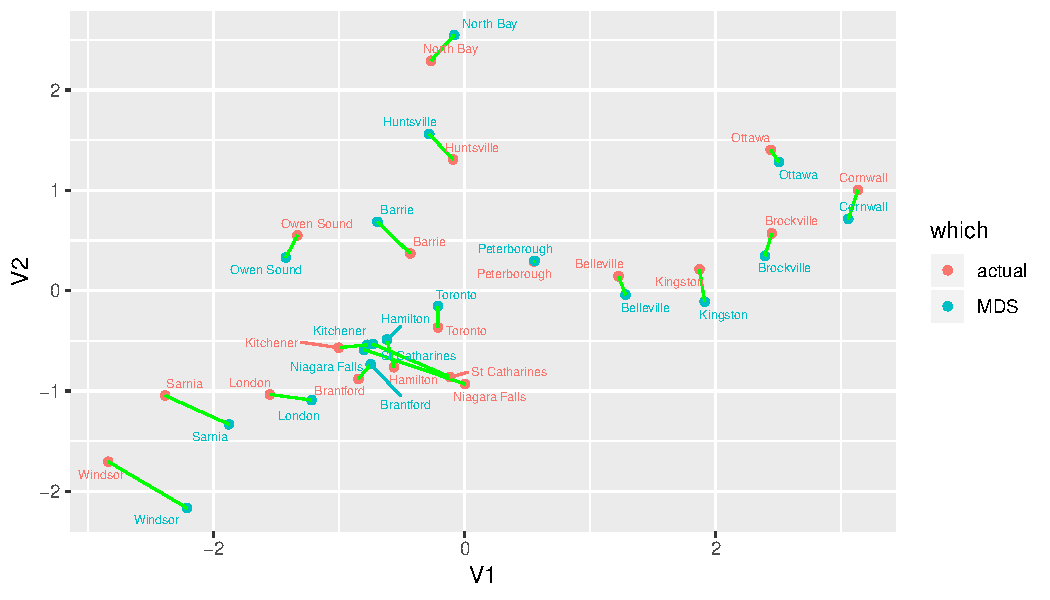
\includegraphics{figure/prosesto-1.pdf}
\caption{plot of chunk prosesto}
\end{figure}

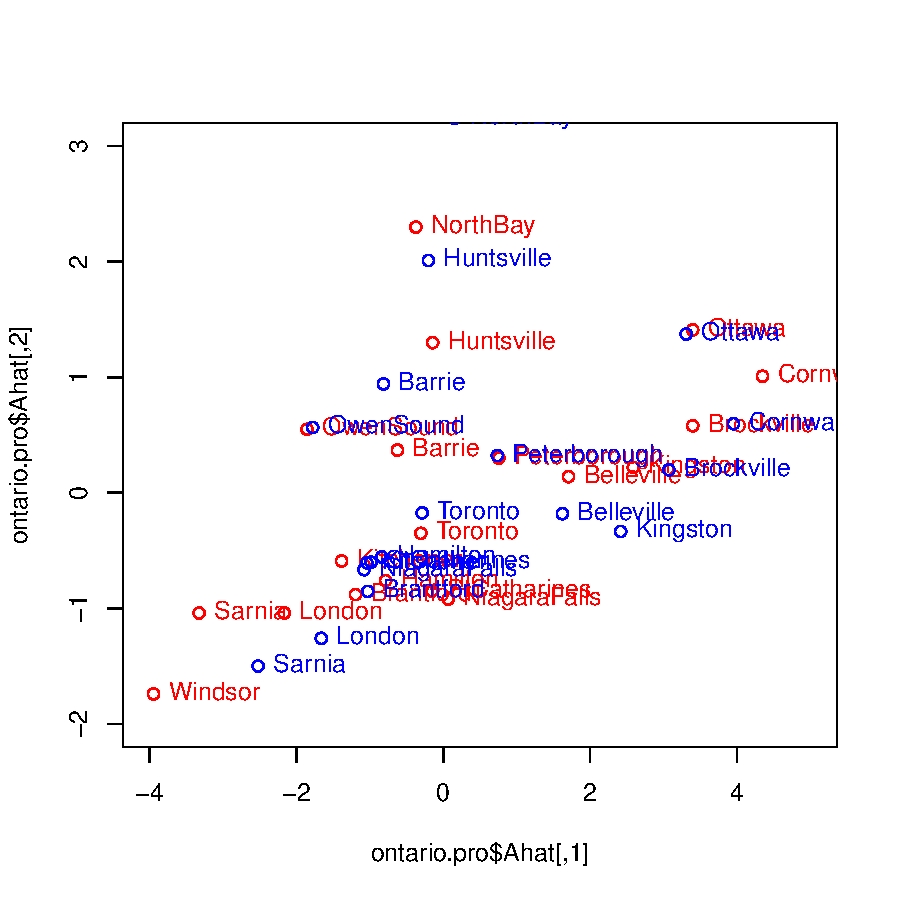
\includegraphics{bMDS-ont-proc.png}

\end{frame}

\begin{frame}[fragile]{Comments}
\protect\hypertarget{comments-2}{}

\begin{itemize}
\item
  True locations red, MDS locations blue
\item
  Most things in roughly right place (esp.~relative to other things)
\item
  Extreme cities off by a bit, but OK relative to neighbours.
\item
  St Catharines, Niagara Falls off by most.
\item
  Sarnia, Windsor also off noticeably.
\item
  These four cities had largest ``third dimension'' in 3D representation
  \texttt{ontario2.3}.
\end{itemize}

\end{frame}

\begin{frame}[fragile]{Rotation matrix}
\protect\hypertarget{rotation-matrix}{}

Shows how MDS map needs to be rotated to get best match with actual
coordinates:

\begin{Shaded}
\begin{Highlighting}[]
\NormalTok{ontario.pro}\OperatorTok{$}\NormalTok{R}
\end{Highlighting}
\end{Shaded}

\begin{verbatim}
##            [,1]      [,2]
## [1,]  0.8845749 0.4663981
## [2,] -0.4663981 0.8845749
\end{verbatim}

Rotation angle \(\theta\) such that \(\cos\theta=0.885\),
\(\sin\theta=0.466\): \(\theta=23\) degrees (counterclockwise). \$ \%\$
\%\$

\end{frame}

\begin{frame}[fragile]{Is that right? Look at MDS map again}
\protect\hypertarget{is-that-right-look-at-mds-map-again}{}

\begin{Shaded}
\begin{Highlighting}[]
\NormalTok{g}
\end{Highlighting}
\end{Shaded}

\begin{figure}
\centering
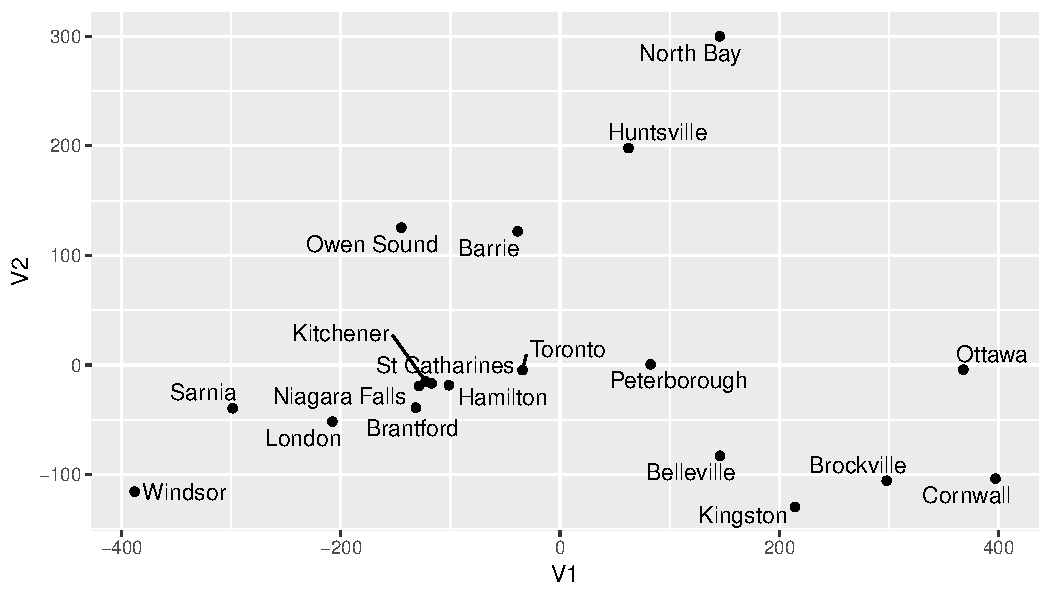
\includegraphics{figure/unnamed-chunk-52-1.pdf}
\caption{plot of chunk unnamed-chunk-52}
\end{figure}

23 degrees counterclockwise seems about right.

\end{frame}

\begin{frame}[fragile]{A cube}
\protect\hypertarget{a-cube}{}

\begin{verbatim}

a-----b
|\    |\
| c---- d
| |   | |
e-|---f |
\|    \|
g-----h
\end{verbatim}

Cube has side length 1, so distance across diagonal on same face is
\(\sqrt{2}\simeq 1.4\) and ``long'' diagonal of cube is
\(\sqrt{3}\simeq 1.7\). \vspace{3ex}

Try MDS on this obviously 3-dimensional data.

\end{frame}

\begin{frame}[fragile]{Cube data as distances xxx}
\protect\hypertarget{cube-data-as-distances-xxx}{}

\footnotesize

\begin{Shaded}
\begin{Highlighting}[]
\NormalTok{my_url <-}\StringTok{ "http://www.utsc.utoronto.ca/~butler/d29/cube.txt"}
\NormalTok{cube <-}\StringTok{ }\KeywordTok{read_delim}\NormalTok{(my_url, }\StringTok{" "}\NormalTok{)}
\NormalTok{cube}
\end{Highlighting}
\end{Shaded}

\begin{verbatim}
## # A tibble: 8 x 9
##   x     `  a` `  b` `  c` `  d` `  e` `   f` ` g`  `  h`
##   <chr> <chr> <chr> <chr> <chr> <chr> <chr>  <chr> <chr>
## 1 a     "  0" " NA" " NA" " NA" " NA" "  NA" <NA>  " NA"
## 2 b     "  1" "  0" " NA" " NA" " NA" "  NA" <NA>  " NA"
## 3 c     "  1" "  1" "  0" " NA" " NA" "  NA" <NA>  " NA"
## 4 d     1.4   "  1" "  1" "  0" " NA" "  NA" <NA>  " NA"
## 5 e     "  1" 1.4   1.4   1.7   "  0" "  NA" <NA>  " NA"
## 6 f     1.4   "  1" 1.7   1.4   "  1" "   0" <NA>  " NA"
## 7 g     1.4   1.7   "  1" 1.4   "  1" " 1.4" " 0"  " NA"
## 8 h     1.7   1.4   1.4   "  1" 1.4   "   1" " 1"  "  0"
\end{verbatim}

\normalsize

\end{frame}

\begin{frame}[fragile]{Making \texttt{dist\ object}}
\protect\hypertarget{making-dist-object}{}

\begin{Shaded}
\begin{Highlighting}[]
\NormalTok{cube.d <-}\StringTok{ }\NormalTok{cube }\OperatorTok\StringTok{ }\KeywordTok{select}\NormalTok{(}\OperatorTok{-}\DecValTok{1}\NormalTok{) }\OperatorTok\StringTok{ }\KeywordTok{as.dist}\NormalTok{()}
\end{Highlighting}
\end{Shaded}

\begin{verbatim}
## Warning in storage.mode(m) <- "numeric": NAs introduced by coercion
\end{verbatim}

\begin{Shaded}
\begin{Highlighting}[]
\NormalTok{cube.d}
\end{Highlighting}
\end{Shaded}

\begin{verbatim}
##        a   b   c   d   e    f   g
##   b  1.0                         
##   c  1.0 1.0                     
##   d  1.4 1.0 1.0                 
##   e  1.0 1.4 1.4 1.7             
##    f 1.4 1.0 1.7 1.4 1.0         
##  g   1.4 1.7 1.0 1.4 1.0  1.4    
##   h  1.7 1.4 1.4 1.0 1.4  1.0 1.0
\end{verbatim}

\end{frame}

\begin{frame}[fragile]{MDS and plotting commands}
\protect\hypertarget{mds-and-plotting-commands}{}

\begin{itemize}
\tightlist
\item
  By default in 2 dimensions; save the extra stuff for later:
\end{itemize}

\begin{Shaded}
\begin{Highlighting}[]
\NormalTok{cube}\FloatTok{.2}\NormalTok{ <-}\StringTok{ }\NormalTok{cube.d }\OperatorTok\StringTok{ }\KeywordTok{cmdscale}\NormalTok{(}\DataTypeTok{eig =}\NormalTok{ T)}
\end{Highlighting}
\end{Shaded}

\begin{itemize}
\tightlist
\item
  Make data frame to plot, remembering the points to plot are in
  \texttt{points} now:
\end{itemize}

\begin{Shaded}
\begin{Highlighting}[]
\NormalTok{d <-}\StringTok{ }\NormalTok{cube}\FloatTok{.2}\OperatorTok{$}\NormalTok{points }\OperatorTok
\StringTok{  }\KeywordTok{as_tibble}\NormalTok{() }\OperatorTok
\StringTok{  }\KeywordTok{mutate}\NormalTok{(}\DataTypeTok{corners =}\NormalTok{ cube}\OperatorTok{$}\NormalTok{x)}
\end{Highlighting}
\end{Shaded}

\begin{itemize}
\tightlist
\item
  Plot points labelled by our names for the corners:
\end{itemize}

\begin{Shaded}
\begin{Highlighting}[]
\NormalTok{g <-}\StringTok{ }\KeywordTok{ggplot}\NormalTok{(d, }\KeywordTok{aes}\NormalTok{(}\DataTypeTok{x =}\NormalTok{ V1, }\DataTypeTok{y =}\NormalTok{ V2, }\DataTypeTok{label =}\NormalTok{ corners)) }\OperatorTok{+}
\StringTok{  }\KeywordTok{geom_point}\NormalTok{() }\OperatorTok{+}\StringTok{ }\KeywordTok{geom_text_repel}\NormalTok{()}
\end{Highlighting}
\end{Shaded}

\end{frame}

\begin{frame}{The ``cube''}
\protect\hypertarget{the-cube}{}

\begin{figure}
\centering

\includegraphics{figure/bianconeri-1.pdf}
\caption{plot of chunk bianconeri}
\end{figure}

Not good.

\end{frame}

\begin{frame}[fragile]{2 and 3 dimensions}
\protect\hypertarget{and-3-dimensions}{}

\begin{Shaded}
\begin{Highlighting}[]
\NormalTok{cube}\FloatTok{.3}\NormalTok{ <-}\StringTok{ }\NormalTok{cube.d }\OperatorTok\StringTok{ }\KeywordTok{cmdscale}\NormalTok{(}\DecValTok{3}\NormalTok{, }\DataTypeTok{eig =}\NormalTok{ T)}
\NormalTok{cube}\FloatTok{.2}\OperatorTok{$}\NormalTok{GOF}
\end{Highlighting}
\end{Shaded}

\begin{verbatim}
## [1] 0.639293 0.664332
\end{verbatim}

\begin{Shaded}
\begin{Highlighting}[]
\NormalTok{cube}\FloatTok{.3}\OperatorTok{$}\NormalTok{GOF}
\end{Highlighting}
\end{Shaded}

\begin{verbatim}
## [1] 0.9143532 0.9501654
\end{verbatim}

\begin{itemize}
\tightlist
\item
  Really need 3rd dimension to represent cube.
\end{itemize}

\end{frame}

\begin{frame}{Non-metric scaling}
\protect\hypertarget{non-metric-scaling}{}

\begin{itemize}
\item
  Sometimes distances not meaningful \emph{as distances}
\item
  Only order matters: closest should be closest, farthest farthest on
  map, but how much further doesn't matter.
\item
  Non-metric scaling, aims to minimize \textbf{stress}, measure of lack
  of fit.
\item
  Example: languages. Make map based on ``similarity'' of number names,
  without requiring that 1 is ``eight times better'' than 8.
\end{itemize}

\end{frame}

\begin{frame}[fragile]{The languages}
\protect\hypertarget{the-languages}{}

\begin{itemize}
\tightlist
\item
  Recall language data (from cluster analysis): 1--10, measure
  dissimilarity between two languages by how many number names
  \emph{differ} xxx in first letter:
\end{itemize}

xxx

\scriptsize

\begin{Shaded}
\begin{Highlighting}[]
\NormalTok{my_url <-}\StringTok{ "http://www.utsc.utoronto.ca/~butler/d29/languages.txt"}
\NormalTok{number.d <-}\StringTok{ }\KeywordTok{read_table}\NormalTok{(my_url)}
\NormalTok{number.d}
\end{Highlighting}
\end{Shaded}

\begin{verbatim}
## # A tibble: 11 x 12
##    la       en    no    dk    nl    de    fr    es
##    <chr> <dbl> <dbl> <dbl> <dbl> <dbl> <dbl> <dbl>
##  1 en        0     2     2     7     6     6     6
##  2 no        2     0     1     5     4     6     6
##  3 dk        2     1     0     6     5     6     5
##  4 nl        7     5     6     0     5     9     9
##  5 de        6     4     5     5     0     7     7
##  6 fr        6     6     6     9     7     0     2
##  7 es        6     6     5     9     7     2     0
##  8 it        6     6     5     9     7     1     1
##  9 pl        7     7     6    10     8     5     3
## 10 hu        9     8     8     8     9    10    10
## 11 fi        9     9     9     9     9     9     9
## # … with 4 more variables: it <dbl>, pl <dbl>,
## #   hu <dbl>, fi <dbl>
\end{verbatim}

\normalsize

\end{frame}

\begin{frame}[fragile]{Non-metric scaling}
\protect\hypertarget{non-metric-scaling-1}{}

\begin{itemize}
\item
  Turn language dissimilarities into \texttt{dist} object
\item
  Run through \texttt{isoMDS} from \texttt{MASS} package; works like
  \texttt{cmdscale}.
\item
  Map only reproduces \emph{relative} xxx closeness of languages. xxx
\end{itemize}

\small

\begin{Shaded}
\begin{Highlighting}[]
\NormalTok{d <-}\StringTok{ }\NormalTok{number.d }\OperatorTok
\StringTok{  }\KeywordTok{select_if}\NormalTok{(is.numeric) }\OperatorTok
\StringTok{  }\KeywordTok{as.dist}\NormalTok{()}
\NormalTok{number.nm <-}\StringTok{ }\NormalTok{d }\OperatorTok\StringTok{ }\KeywordTok{isoMDS}\NormalTok{()}
\end{Highlighting}
\end{Shaded}

\begin{verbatim}
## initial  value 12.404671 
## iter   5 value 5.933653
## iter  10 value 5.300747
## final  value 5.265236 
## converged
\end{verbatim}

\begin{Shaded}
\begin{Highlighting}[]
\KeywordTok{names}\NormalTok{(number.nm)}
\end{Highlighting}
\end{Shaded}

\begin{verbatim}
## [1] "points" "stress"
\end{verbatim}

\normalsize

\begin{itemize}
\tightlist
\item
  \texttt{points} for plotting, \texttt{stress} measure of fit (lower
  better).
\end{itemize}

\end{frame}

\begin{frame}[fragile]{Results}
\protect\hypertarget{results}{}

\begin{itemize}
\tightlist
\item
  Stress is very low (5\%, good):
\end{itemize}

\begin{Shaded}
\begin{Highlighting}[]
\NormalTok{number.nm}\OperatorTok{$}\NormalTok{stress}
\end{Highlighting}
\end{Shaded}

\begin{verbatim}
## [1] 5.265236
\end{verbatim}

\$ \%\$ \%\$

\begin{itemize}
\tightlist
\item
  Familiar process: make a data frame to plot. Use name \texttt{dd} for
  data frame this time since used \texttt{d} for distance object:
\end{itemize}

\begin{Shaded}
\begin{Highlighting}[]
\NormalTok{dd <-}\StringTok{ }\NormalTok{number.nm}\OperatorTok{$}\NormalTok{points }\OperatorTok
\StringTok{  }\KeywordTok{as_tibble}\NormalTok{() }\OperatorTok
\StringTok{  }\KeywordTok{mutate}\NormalTok{(}\DataTypeTok{lang =}\NormalTok{ number.d}\OperatorTok{$}\NormalTok{la)}
\end{Highlighting}
\end{Shaded}

\begin{itemize}
\tightlist
\item
  Make plot:
\end{itemize}

\begin{Shaded}
\begin{Highlighting}[]
\NormalTok{g <-}\StringTok{ }\KeywordTok{ggplot}\NormalTok{(dd, }\KeywordTok{aes}\NormalTok{(}\DataTypeTok{x =}\NormalTok{ V1, }\DataTypeTok{y =}\NormalTok{ V2, }\DataTypeTok{label =}\NormalTok{ lang)) }\OperatorTok{+}
\StringTok{  }\KeywordTok{geom_point}\NormalTok{() }\OperatorTok{+}\StringTok{ }\KeywordTok{geom_text_repel}\NormalTok{()}
\end{Highlighting}
\end{Shaded}

\end{frame}

\begin{frame}{The languages map}
\protect\hypertarget{the-languages-map}{}

\begin{figure}
\centering
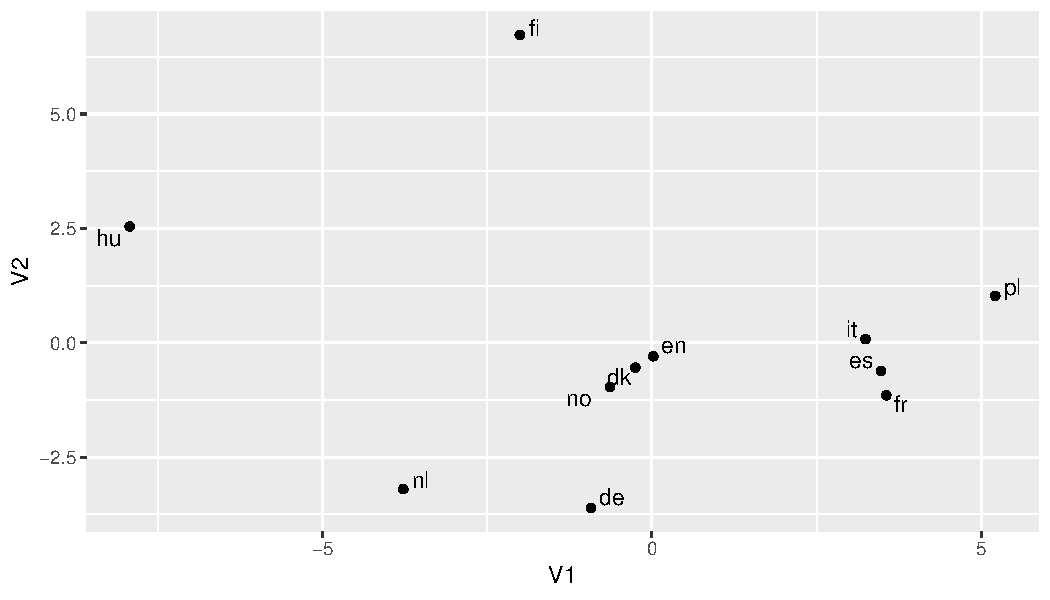
\includegraphics{figure/padova-1.pdf}
\caption{plot of chunk padova}
\end{figure}

\end{frame}

\begin{frame}{Comments}
\protect\hypertarget{comments-3}{}

\begin{itemize}
\item
  Tight clusters: Italian-Spanish-French, English-Danish-Norwegian.
\item
  Dutch and German close to English group.
\item
  Polish close to French group.
\item
  Hungarian, Finnish distant from everything else and each other!
\item
  Similar conclusions as from the cluster analysis.
\end{itemize}

\end{frame}

\begin{frame}{Shepard diagram}
\protect\hypertarget{shepard-diagram}{}

\begin{itemize}
\item
  Stress for languages data was 5.3\%, very low.
\item
  How do observed dissimilarities and map distances correspond?
\item
  For low stress, expect larger dissimilarity to go with larger map
  distance, almost all the time.
\item
  Not necessarily a linear trend since non-metric MDS works with
  \emph{order} of values.
\item
  Actual dissimilarity on \(x\)-axis; map distances on \(y\)-axis.
\end{itemize}

\end{frame}

\begin{frame}[fragile]{Shepard diagram for languages}
\protect\hypertarget{shepard-diagram-for-languages}{}

\begin{Shaded}
\begin{Highlighting}[]
\KeywordTok{Shepard}\NormalTok{(d, number.nm}\OperatorTok{$}\NormalTok{points) }\OperatorTok
\StringTok{  }\KeywordTok{as_tibble}\NormalTok{() }\OperatorTok
\StringTok{  }\KeywordTok{ggplot}\NormalTok{(}\KeywordTok{aes}\NormalTok{(}\DataTypeTok{x =}\NormalTok{ x, }\DataTypeTok{y =}\NormalTok{ y)) }\OperatorTok{+}\StringTok{ }\KeywordTok{geom_point}\NormalTok{()}
\end{Highlighting}
\end{Shaded}

\begin{figure}
\centering
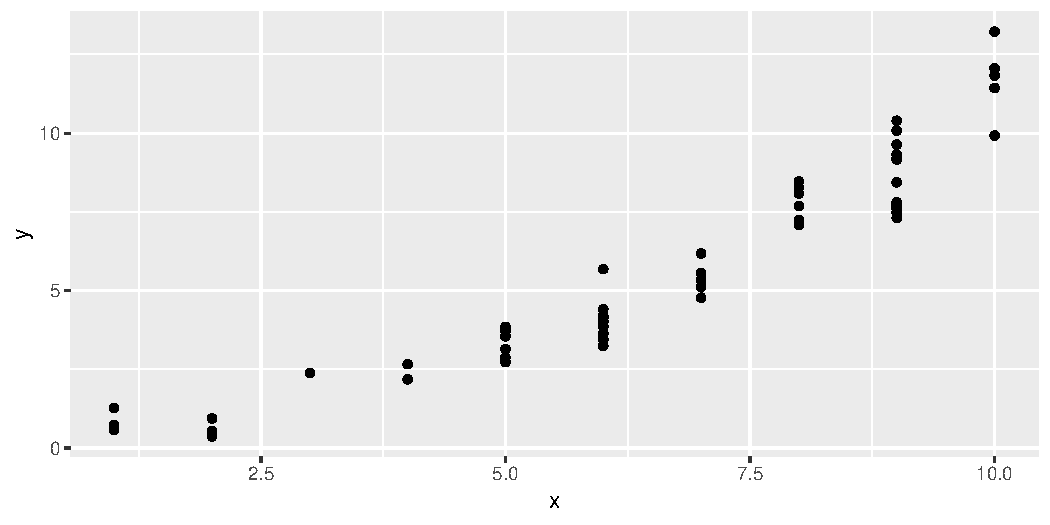
\includegraphics{figure/parma-1.pdf}
\caption{plot of chunk parma}
\end{figure}

Actual dissimilarity \(x\) between higher: mapped distance \(y\) from
MDS higher too. (MDS working well.)

\end{frame}

\begin{frame}[fragile]{Cube, revisited xxx}
\protect\hypertarget{cube-revisited-xxx}{}

\small

\begin{Shaded}
\begin{Highlighting}[]
\NormalTok{cube.d <-}\StringTok{ }\NormalTok{cube }\OperatorTok\StringTok{ }\KeywordTok{select}\NormalTok{(}\OperatorTok{-}\NormalTok{x) }\OperatorTok\StringTok{ }\KeywordTok{as.dist}\NormalTok{(cube)}
\end{Highlighting}
\end{Shaded}

\begin{verbatim}
## Warning in storage.mode(m) <- "numeric": NAs introduced
## by coercion
\end{verbatim}

\begin{Shaded}
\begin{Highlighting}[]
\NormalTok{cube}\FloatTok{.2}\NormalTok{ <-}\StringTok{ }\KeywordTok{isoMDS}\NormalTok{(cube.d, }\DataTypeTok{trace =}\NormalTok{ F)}
\NormalTok{cube}\FloatTok{.2}\OperatorTok{$}\NormalTok{stress}
\end{Highlighting}
\end{Shaded}

\begin{verbatim}
## [1] 17.97392
\end{verbatim}

\begin{Shaded}
\begin{Highlighting}[]
\NormalTok{cube}\FloatTok{.3}\NormalTok{ <-}\StringTok{ }\KeywordTok{isoMDS}\NormalTok{(cube.d, }\DataTypeTok{k =} \DecValTok{3}\NormalTok{, }\DataTypeTok{trace =}\NormalTok{ F)}
\NormalTok{cube}\FloatTok{.3}\OperatorTok{$}\NormalTok{stress}
\end{Highlighting}
\end{Shaded}

\begin{verbatim}
## [1] 0.007819523
\end{verbatim}

\normalsize

\begin{itemize}
\item
  Stress is 18\% for 2 dimensions, basically 0\% for 3.
\item
  Three dimensions correct, two dimensions bad.
\item
  Shepard diagrams for these: xxx
\end{itemize}

\footnotesize

\begin{Shaded}
\begin{Highlighting}[]
\NormalTok{cube2.sh <-}\StringTok{ }\KeywordTok{Shepard}\NormalTok{(cube.d, cube}\FloatTok{.2}\OperatorTok{$}\NormalTok{points)}
\NormalTok{g2 <-}\StringTok{ }\KeywordTok{ggplot}\NormalTok{(}\KeywordTok{as.data.frame}\NormalTok{(cube2.sh), }\KeywordTok{aes}\NormalTok{(}\DataTypeTok{x =}\NormalTok{ x, }\DataTypeTok{y =}\NormalTok{ y)) }\OperatorTok{+}
\StringTok{  }\KeywordTok{geom_point}\NormalTok{()}
\NormalTok{cube3.sh <-}\StringTok{ }\KeywordTok{Shepard}\NormalTok{(cube.d, cube}\FloatTok{.3}\OperatorTok{$}\NormalTok{points)}
\NormalTok{g3 <-}\StringTok{ }\KeywordTok{ggplot}\NormalTok{(}\KeywordTok{as.data.frame}\NormalTok{(cube3.sh), }\KeywordTok{aes}\NormalTok{(}\DataTypeTok{x =}\NormalTok{ x, }\DataTypeTok{y =}\NormalTok{ y)) }\OperatorTok{+}
\StringTok{  }\KeywordTok{geom_point}\NormalTok{()}
\end{Highlighting}
\end{Shaded}

\normalsize

\end{frame}

\begin{frame}[fragile]{Shepard diagram for 2-dimensional cube}
\protect\hypertarget{shepard-diagram-for-2-dimensional-cube}{}

\begin{Shaded}
\begin{Highlighting}[]
\NormalTok{g2}
\end{Highlighting}
\end{Shaded}

\begin{figure}
\centering
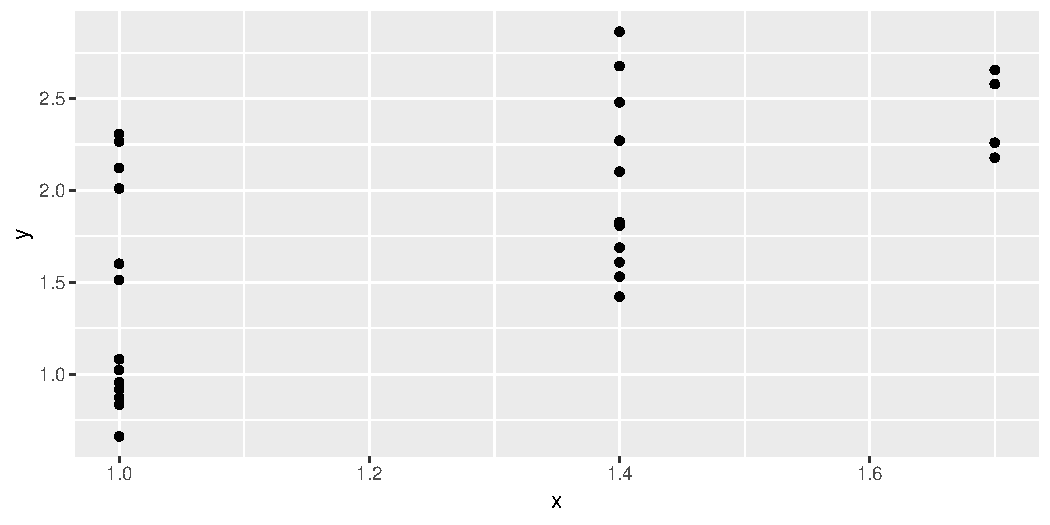
\includegraphics{figure/unnamed-chunk-65-1.pdf}
\caption{plot of chunk unnamed-chunk-65}
\end{figure}

Poor correspondence (not much trend).

\end{frame}

\begin{frame}[fragile]{Shepard diagram for 3-dimensional cube}
\protect\hypertarget{shepard-diagram-for-3-dimensional-cube}{}

\begin{Shaded}
\begin{Highlighting}[]
\NormalTok{g3}
\end{Highlighting}
\end{Shaded}

\begin{figure}
\centering
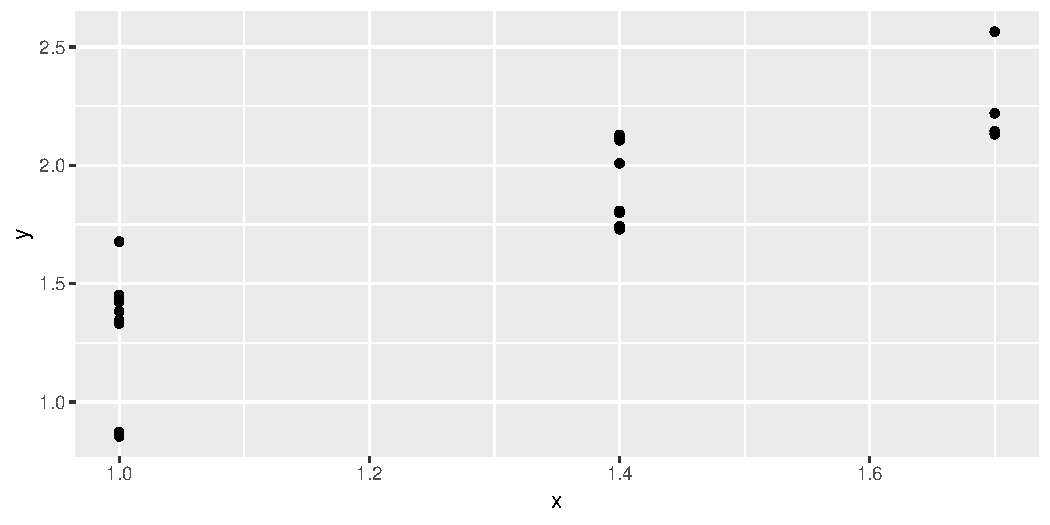
\includegraphics{figure/unnamed-chunk-66-1.pdf}
\caption{plot of chunk unnamed-chunk-66}
\end{figure}

Almost perfect: all actual \(x=1\) go with smallest mapped distances;
almost all \(x=1.7\) go with largest.

\end{frame}

\begin{frame}{Guidelines for stress values, in \%}
\protect\hypertarget{guidelines-for-stress-values-in}{}

Smaller is better:

\begin{tabular}{lp{3in}}
Stress value & Interpretation \\
\hline
Less than 5 & Excellent: no prospect of misinterpretation (rarely achieved)\\
5--10 & Good: most distances reproduced well, small prospect of false inferences\\
10--20 & Fair: usable, but some distances misleading.\\
More than 20 & Poor: may be dangerous to interpret\\
\hline
\end{tabular}

\begin{itemize}
\item
  Languages: stress in ``good'' range.
\item
  Cube: xxx

  \begin{itemize}
  \item
    2 dimensions ``fair'', almost ``poor'';
  \item
    3 dimensions, ``excellent''.
  \end{itemize}
\end{itemize}

\end{frame}

\end{document}
